\documentclass[11pt]{article}
\usepackage[T1]{fontenc}
\usepackage[utf8]{inputenc}
\usepackage{lmodern,microtype}
\usepackage[margin=1in]{geometry}
\usepackage{amsmath,amssymb,amsthm,mathtools}
\usepackage{graphicx,booktabs,tabularx,array}
\newcolumntype{Y}{>{\raggedright\arraybackslash}X}
\newcolumntype{P}[1]{>{\raggedright\arraybackslash}p{#1}}
\usepackage[dvipsnames]{xcolor}
\usepackage{enumitem}
\usepackage{fancyhdr}
\usepackage{hyperref}
\hypersetup{colorlinks=true,linkcolor=MidnightBlue,citecolor=MidnightBlue,
  urlcolor=MidnightBlue,pdftitle={Robust Choices That Never Settle},
  pdfauthor={Research article prepared for Vladimir Reshetnikov}}
\urlstyle{same}
\setlength{\emergencystretch}{2em}
\setlength{\headheight}{14pt}
\pagestyle{fancy}
\fancyhf{}
\fancyhead[L]{\small Robust Choices That Never Settle}
\fancyhead[R]{\small Finite and infinite forms}
\fancyfoot[C]{\thepage}
\setlist{itemsep=3pt,topsep=6pt}
\newtheorem{theorem}{Theorem}[section]
\newtheorem{lemma}[theorem]{Lemma}
\newtheorem{proposition}[theorem]{Proposition}
\newtheorem{corollary}[theorem]{Corollary}
\theoremstyle{definition}
\newtheorem{definition}[theorem]{Definition}
\newtheorem{problem}[theorem]{Problem}
\theoremstyle{remark}
\newtheorem{remark}[theorem]{Remark}
\newcommand{\E}{\mathbb E}
\newcommand{\Prb}{\mathbb P}
\newcommand{\N}{\mathbb N}
\newcommand{\R}{\mathbb R}
\newcommand{\F}{\mathbb F}
\newcommand{\Qn}{\{-1,1\}^{n}}
\newcommand{\Om}{\{-1,1\}^{\N}}
\newcommand{\cF}{\mathcal F}
\newcommand{\eps}{\varepsilon}
\newcommand{\Maj}{\operatorname{Maj}}
\newcommand{\diam}{\operatorname{diam}}
\newcommand{\TV}{\operatorname{TV}}
\newcommand{\one}{\mathbf 1}
\newcommand{\dist}{d_H}
\newcommand{\Ball}{\mathcal B}
\newcommand{\vol}{V}
\newcommand{\flip}{\tau}
\newcommand{\neutral}{\mathcal N}
\newcommand{\code}[1]{\texttt{\detokenize{#1}}}
\DeclareMathOperator{\Inf}{Inf}
% Added by the ProveIt write phase (batch 114, 5 October 2026): dated notes
% marked [write].
\newcommand{\file}[1]{\nolinkurl{#1}}
\newenvironment{writenote}[1][]{\par\smallskip\begingroup\small
 \noindent\textbf{[write]}\if\relax\detokenize{#1}\relax\else~\textbf{#1.}\fi\ }%
 {\par\endgroup\smallskip}

\title{\textbf{Robust Choices That Never Settle}\\[5pt]
  \large An exact finite--infinite puzzle about resilience, choice, and randomness}
\author{Research article prepared for Vladimir Reshetnikov}
\date{5 October 2026}

\begin{document}
\maketitle
\begin{abstract}
A committee must choose one of two alternatives, treat their names symmetrically,
and withstand adversarial changes to its votes. How robust can a finite rule be,
and can increasingly robust finite rules settle into a neutral infinite rule?
We solve the finite optimization exactly by an antipodal-core reduction to
Kleitman's diameter theorem: odd majority simultaneously maximizes every Hamming
robustness probability, and an even committee has the same optimum as a committee
with one fewer member. We then prove a sharp finite-prefix inequality converting
adversarial vulnerability into conditional predictability. Its optimal constant
is the reciprocal of a Hamming-ball volume fraction. The inequality shows that
even vanishing one-vote vulnerability forces the decisions to disagree
asymptotically half the time with every fixed measurable candidate limit.
They oscillate on a conull, comeager set.

For stronger resilience, we extract a deterministic sequence of committee sizes
whose decision map is a continuous open surjection with output law arbitrarily
close, in a bounded-density sense, to fair Bernoulli measure. Along these sizes,
robustness tends to infinity and decisions are statistically normal almost
surely, whereas generically the frequencies swing from zero to one and
one-vote fragility recurs. An everywhere neutral infinite rule nevertheless
exists under choice, with maximally nonmeasurable fibres. For biased product
laws, completed-measure existence has an exact square-summability threshold.
The article includes complete proofs of the derived statements, explicit
separations, an exact finite verifier, a ProveIt integration map, and further
research questions. Classical ingredients and unverified priority claims are
carefully distinguished.
\end{abstract}

\noindent\textbf{Keywords.} Boolean functions; Hamming robustness; Kleitman diameter
theorem; mixing convergence; finite-change equivalence; Baire category; choice.

\begin{writenote}[Status and trust boundary, added 5 October 2026, batch~114]
This is an unrefereed external manuscript, filed in ProveIt as the
single-source research report \file{robust-neutral-choice} (provenance, the
sources as the write read them, relation to the repository, the collected
non-claims and the reading conventions are in
Section~\ref{rch:sec:provenance}). Its author line and its PDF author field
read ``Research article prepared for Vladimir Reshetnikov''; the package
says nothing about how the text was produced, and the write adds no
authorship statement. No statement of the report is formalized in Lean or
Rocq (Remark~\ref{rch:rem:lean} says which proved Lean declarations bear on
the category half of Theorem~\ref{rch:thm:choice}).
\emph{What rests on what.} The finite optimum,
Theorem~\ref{rch:thm:finite}, is a corollary of Kleitman's diameter theorem
(Theorem~\ref{rch:thm:kleitman}, quoted without proof and credited, as the
source credits it, to~\cite{Kleitman,HKP}); the source proves the
antipodal-core reduction (Lemma~\ref{rch:lem:core}) and the matching
majority construction, and claims no novelty for the optimum.
Theorem~\ref{rch:thm:bias} takes Kakutani's product-measure
dichotomy~\cite{Kakutani} as an explicit input. Every other theorem,
lemma and proposition of the source is proved in the text from standard probability, measure theory
and topology (the central limit theorem and Stirling's formula in
Proposition~\ref{rch:prop:scales}; conditional expectations, Borel--Cantelli,
Radon--Nikodym and compactness later); the mixing conclusions are
consequences of R\'enyi's theory of mixing sequences~\cite{Renyi} and the
sparse extraction belongs to the subsequence-principle
literature~\cite{Aldous,AldousEagleson}, both credited by the source. The
exhaustive program \file{code/verify.py} checks the finite statements in
dimensions one to five and proves nothing in higher dimension. The source
claims no novelty or priority and does not claim to settle a published open
problem. The write adds Remark~\ref{rch:rem:lean},
Proposition~\ref{rch:prop:alphabet} (the regularity obstruction for more
than two labels), short notes marked [write] and
Section~\ref{rch:sec:further}.
\end{writenote}

\newpage
\tableofcontents
\newpage

\section{The problem and its mathematical setting}
\label{rch:sec:problem}

Imagine a committee receiving a binary vote from each member. A rule must always
return a decision. Renaming the two alternatives must rename the decision too.
After the votes are cast, an adversary sees the entire configuration and may
change up to \(r\) votes. We ask how often the original decision survives
\emph{every} such intervention. The votes are fair and independent only for
measuring the fraction of robust inputs; the intervention itself is worst case.

Now let a single infinite stream of votes feed committees of increasing size.
Suppose each fixed intervention budget becomes harmless with probability tending
to one. It is tempting to expect an eventually settled decision, insensitive to
finite alterations of the stream. The principal surprise is that the two
requirements pull in different directions: improving resilience can erase the
influence of every fixed initial segment without producing a measurable limit.

\begin{problem}[Robust neutral choice]
\label{rch:prob:main}
Answer the following linked questions.
\begin{enumerate}[label=(\roman*)]
\item For \(n\) fair binary inputs, what is the largest fraction on which a
neutral deterministic rule withstands all changes to at most \(r\) coordinates?
Can one rule attain the optimum for every \(r\)?
\item Can neutral rules on growing prefixes become resistant to every fixed
number of changes and nevertheless converge on a substantial set of streams?
\item If convergence is impossible, how much randomness and how much
topological freedom remain in the sequence of decisions?
\item Can a perfectly robust neutral rule be defined directly on infinite
streams? How do choice and measurability affect the answer?
\end{enumerate}
\end{problem}

\subsection{Why this problem fits the requested intersection}

Epoch AI's public biographical note describes Elliot Glazer's interests as set
theory and formal systems, choice paradoxes, proof-assistant foundations, and
puzzles with finite and infinite versions \cite{Epoch}. His dissertation
\emph{Interactions Among Principles of Choice, Forcing, and Measure Theory}
examines the relation between choice and regularity, including transversals of
Borel equivalence relations \cite{Glazer}. These sources support the proposed
fit; the problem has not been reviewed or endorsed by him.

ProveIt provides a concrete starting point. Its
\code{GenericErgodicity.lean} develops finite-change generic ergodicity and
obstructions to regular finite-label rules. The abstract theorems
\code{generic_const} and \code{fixed_label}, together with
\code{Cantor.transitive}, supply the category mechanism used here
\cite{ProveIt}. The present question adds exact finite robustness and a
quantitative analysis of what finite approximations can do. Section
\ref{rch:sec:formal} identifies the precise existing ingredients and the additional
formalization tasks.

\subsection{Definitions and conventions}

Write \(Q_n=\{-1,1\}^n\), with uniform probability \(\mu_n\), and let
\(\dist\) denote Hamming distance. Complementation is \(x\mapsto -x\).

\begin{definition}
A rule \(f:Q_n\to\{-1,1\}\) is \emph{neutral}, or self-dual, if
\begin{equation}
 f(-x)=-f(x) \qquad(x\in Q_n).
 \label{rch:eq:neutral}
\end{equation}
Its \emph{change distance} is
\begin{equation}
 R_f(x)=\min\{\dist(x,y): f(y)\ne f(x)\}.
 \label{rch:eq:radius}
\end{equation}
For an integer \(r\ge0\), define
\begin{equation}
 \rho_f(r)=\mu_n(R_f>r),\qquad
 \eps_f(r)=1-\rho_f(r)=\mu_n(R_f\le r).
 \label{rch:eq:profiles}
\end{equation}
Thus \(R_f\ge1\), and \(R_f=1\) means that a single vote can change the answer.
\end{definition}

Neutrality implies that \(f\) is balanced: its two fibres have equal size.
It does not require invariance under permutations of voters. We use the term
\emph{neutral}, not \emph{anonymous}, for this reason. For odd committees,
the optimal majority rule is anonymous as well. For an even committee, a neutral
anonymous deterministic rule cannot exist: a tied configuration and its
complement are permutations of one another, but neutrality demands opposite
outputs.

On \(\Omega=\Om\), let \(\mu\) be fair product measure and let
\(\cF_m=\sigma(X_1,\ldots,X_m)\). A finite rule is also viewed as a function on
\(\Omega\) by ignoring coordinates after its horizon. We write
\(x\mathrel{E_0}y\) when the two streams differ at only finitely many positions.
All measure-theoretic statements allow the completion of the displayed product
measure. ``Comeager'' means that the complement is a countable union of nowhere
dense sets in the usual Cantor topology.

\subsection{What is classical, what is proved here, and what remains open}

This is a designed problem with a rigorous solution, rather than a claim to have
settled a previously advertised major conjecture. The finite extremum is a
corollary of Kleitman's classical theorem \cite{Kleitman,HKP}. The nonconvergence
mechanism belongs to R\'enyi's theory of mixing sequences \cite{Renyi}; sparse
extraction belongs to the wider subsequence-principle literature
\cite{Aldous,AldousEagleson}. We give direct proofs specialized to the puzzle.

The sharp prefix inequality, its matching examples, the quantitative open
recoding theorem, and the assembled probability/category consequences are
proved below. Their proofs do not certify historical priority. The two substantial
theorems quoted without proof are the explicitly stated diameter theorem and,
in the optional biased extension, Kakutani's product-measure dichotomy. No new
Lean verification is claimed. The further questions in Section
\ref{rch:sec:questions} are research proposals, with their status qualified there.

\subsection{Provenance, sources and reading conventions}
\label{rch:sec:provenance}
\begin{writenote}[Added 5 October 2026, batch~114]
\emph{Provenance.} The report is built from one manuscript, the archive
\file{robust_choices.zip} (617{,}494 bytes; wrapper directory
\file{robust_choices/}, 12 files), which reached ProveIt's
\file{docs/incoming} in the arrival commit \file{2399df2bd} (5~October 2026,
``New research reports''), outside the session bundle of the intake, and
was placed as batch~114 in \file{99053b5d1}. The text is the delivered
\file{robust_choices.tex} (1{,}539 lines), shipped as \file{article.tex};
the delivered code, data and figure files are shipped unchanged (the README
lists them). The delivered 22-page PDF is not shipped; it and the delivery
README (staged at placement and replaced by the report README) are
retrievable from the arrival commit. The package pins ProveIt revision
\file{3b9458b31f459b480ab43a068d7cc56f4cfdbb28}
(Section~\ref{rch:sec:formal}, bibliography entry~\cite{ProveIt} and the
delivery README); that commit is the batch-98D placement commit of this
repository and an ancestor of the commit this write is based on. The author
line and the PDF author field read ``Research article prepared for Vladimir
Reshetnikov''. The package contains no statement of how the text was
produced, no ``unrefereed'' or ``prepared for private review'' line, no
checksum manifest and no personal data. Single source: no merge choice was
made. The write prefixed the 79 delivered labels with \file{rch:} and
updated every reference; it added the notes marked [write], this
subsection, Remark~\ref{rch:rem:lean}, Section~\ref{rch:sec:further} with
Proposition~\ref{rch:prop:alphabet}, and nothing else. No statement, proof
or number of the source was changed: the added remark and proposition are
the only numbered statements of their sections and the added displays are
unnumbered, so every delivered theorem and equation keeps its number.

\emph{The sources, as the write read them} (5~October 2026).
\begin{itemize}\raggedright
\item Huang, Klurman and Pohoata~\cite{HKP}, arXiv version~1: their
 Theorem~1.1 is Theorem~\ref{rch:thm:kleitman} as printed here (both
 parities, diameter at most $D<n$, both bounds sharp, the same extremal
 sets), credited to Kleitman as the solution of a conjecture of Erd\H{o}s;
 the paper gives a new, algebraic proof. Read.
\item Kleitman~\cite{Kleitman}: the bibliographic data were confirmed through
 the DOI; the paper itself was not read.
\item Wu, Li, Feng, Liu and Yu~\cite{WuEtAl}: abstract of version~2 (10~June
 2025) read. It states Kleitman's theorem with the odd bound in the form
 $\sum_{i\le s}\binom ni+\binom{n-1}s$, credits Frankl (2017) with the
 characterization of the extremal families and a first stability result,
 and proves a second one; it concerns extremal families of a given
 diameter, as Question~Q2 says. The body was not read.
\item Kakutani~\cite{Kakutani}, R\'enyi~\cite{Renyi}, Aldous~\cite{Aldous},
 Aldous and Eagleson~\cite{AldousEagleson}: not read by the write. The
 statement used in Section~\ref{rch:sec:bias}, equivalence of the two
 product measures exactly when the product \eqref{rch:eq:kakutani} is
 positive, is the usual form of Kakutani's dichotomy for these products.
\item Epoch AI's biographical note~\cite{Epoch} and Glazer's
 dissertation~\cite{Glazer}: motivation only, not read by the write. The
 source says that the problem has not been reviewed or endorsed by Glazer.
\item The repository at the pin and at the write's base commit: see the note
 in Section~\ref{rch:sec:formal}.
\end{itemize}

\emph{What was checked at intake.} The batch-114 dossier read the manuscript
in full and checked the diameter bound $n-2r-1$ of the core and both
parities of the reduction to Kleitman's theorem, the nine-voter row, the
induction of Lemma~\ref{rch:lem:minboundary}, the fibre cancellation, the
sharpness sandwich \eqref{rch:eq:sharpsandwich}, the code construction
(complement invariance needs $\sum_{v\ne0}v=0$, true for $d\ge2$), the
likelihood product bounds, openness by nested compactness, the singular
case $A'=A\setminus\kappa A$ of Theorem~\ref{rch:thm:bias} and the example
$\gamma\le1/2$; no error. Independent programs confirmed the nine-voter row
exactly and brute-forced the construction of
Proposition~\ref{rch:prop:code} for $d=2$, $N=3$ with $L=1$ and $L=3$: the
rule is neutral, $R_f\le2$ everywhere, and
$\eps_f(1)=u_N+t_L-u_Nt_L$ exactly. The delivered verifier passed on a
copy, and its four outputs equal the shipped data files up to newline style
(the CSV byte for byte). The write reread every proof, found no error, and
made the two exhaustive computations reported in
Section~\ref{rch:sec:further}.

\emph{Relation to the repository.}
\begin{itemize}\raggedright
\item \emph{Formal status.} No statement of this report is formalized in
 Lean or Rocq, and its place in the collection confers no formal status.
 The Lean file the source cites,
 \path{SetTheory/Cardinals/Cardinals/Countable/GenericErgodicity.lean},
 proves the topological zero-one law and its two corollaries that the
 category half of Theorem~\ref{rch:thm:choice} needs;
 Remark~\ref{rch:rem:lean} assembles them and names what is missing.
\item The large-cardinal synthesis
 (\path{SetTheory/Cardinals/docs/cardinals/research-synthesis/}),
 Proposition~15.3, \file{prop:baire} (the Baire-measurable classification of finite-label rules
 at $\lambda=\omega$), is what that Lean file formalizes; its discussion
 notes that a selection from a quotient of $E_0$ type cannot be Baire
 measurable, the mechanism of the category half of
 Theorem~\ref{rch:thm:choice}. There the symmetries are permutations of
 coordinates; here the symmetry is global complementation.
\item \file{noisy-parity-cubes} (same collection and batch; \emph{see
 also}): a total parity label there changes sign under every
 \emph{single} flip and is nonmeasurable for fair measure
 (\file{np:found:choice}, \file{np:found:regularity}); a rule here is
 \emph{invariant} under finite changes and changes sign under global
 complementation. The biased thresholds differ accordingly: every parity
 label is measurable for the product of Bernoulli$(q_i)$ laws exactly when
 $\sum_i\min(q_i,1-q_i)<\infty$ (\file{np:found:biased}), whereas a
 measurable rule of the present kind exists exactly when
 $\sum_i(p_i-\frac12)^2=\infty$ (Theorem~\ref{rch:thm:bias}). Neither
 source cites the other; no theorem is shared.
\item Batch~114 also filed \file{freiling-symmetry-blacklists},
 \file{bounded-width-power-set-compression} and
 \file{random-bits-arithmetic-cuts} in the same category, and
 \file{measurable-box-games} shares the motivation from Glazer's work; no
 theorem is shared with any of them.
\item \emph{Stale claims.} The source's three statements about the repository
 (what \file{GenericErgodicity.lean} contains, the role of
 \file{FiniteCycles.lean}, and that targeted searches did not find the
 quantitative development) are still correct at the write's base commit
 (note in Section~\ref{rch:sec:formal}); nothing needed correcting.
\end{itemize}
\end{writenote}

\begin{writenote}[What is not claimed, collected from the source]
The problem is designed; the source does not claim to have settled ``a
previously advertised major conjecture'', its proofs ``do not certify
historical priority'', and its delivery README says that it ``makes no
unverified claim of worldwide novelty or a breakthrough on a published open
problem''. The finite optimum is a corollary of Kleitman's theorem, quoted
without proof; Theorem~\ref{rch:thm:bias} is ``a deduction from a classical
product-measure theorem, not a new version of Kakutani's theorem'', concerns
existence in one completed biased law and gives no universally measurable
neutral selector. The mixing mechanism is R\'enyi's and sparse extraction
belongs to the subsequence-principle literature; the source gives direct
proofs specialized to the puzzle. No new Lean or Rocq verification is
claimed; the exact finite program is a check, not a proof of the
infinite-dimensional theorems, and its tables for larger $n$ evaluate the
formula rather than enumerate rules. Equation \eqref{rch:eq:plateau} is not
a claim about every fairness criterion or voting model; the attaining rules
are not classified. The constant of Theorem~\ref{rch:thm:prefix} is sharp
only uniformly over dimensions, not for each fixed $(n,m,r)$. In
\eqref{rch:eq:nooracle} the candidate $G$ is fixed before the limit; nothing
is uniform over $G$ depending on $n$, and selecting a constant-sign
subsequence after seeing the input is not excluded.
Proposition~\ref{rch:prop:influences} says nothing about small coalitions.
The selected outputs of Theorem~\ref{rch:thm:recoding} need not be
independent (equivalence with product measure is the claim); the coupling
lives on an enlarged probability space and does not provide an independent
sequence as a function of the input. \eqref{rch:eq:E0hom} is a homomorphism
of equivalence relations on $E$, not a reduction, and $H|_E$ is not claimed
open or onto. The choice construction does not identify the existence of
the rule with full choice, and its exact weak-choice strength is left open.
The Lean declarations should not be reported as ``an already named, directly
matching repository theorem''; the repository searches are ``evidence about
the inspected material, not a certification of novelty''. The explicit
majority schedule is not proposed as optimal. The research questions are
proposals; a question labelled a target is not asserted to be a previously
published open problem. Randomized rules must be neutral for each fixed seed.
The problem has not been reviewed or endorsed by Glazer.
\end{writenote}

\begin{writenote}[Reading conventions]
The abstract's ``For stronger resilience, we extract'' covers more than it
needs: the open map and the bounded density of
Theorem~\ref{rch:thm:recoding} need only one-vote resilience
\eqref{rch:eq:oneassumption}; resilience at every fixed budget
\eqref{rch:eq:allassumption} is the hypothesis of
\eqref{rch:eq:radiusdiverge} and of Theorem~\ref{rch:thm:typical}. The
cube is $\{-1,1\}^n$ throughout the text, but
Proposition~\ref{rch:prop:code} uses $\F_2$ coordinates and the delivered
program uses $\{0,1\}^n$ with outputs $\pm1$ and the first $m$ coordinates as
the low bits. The source reuses letters as follows; no symbol was renamed.
\end{writenote}
\begin{center}\small
\renewcommand{\arraystretch}{1.12}
\begin{tabularx}{\textwidth}{@{}P{0.16\textwidth}YP{0.27\textwidth}@{}}
\toprule
Symbol & Meaning here (where) & Not to be read as\\
\midrule
\emph{neutral}, $R_f$ & self-dual, \eqref{rch:eq:neutral}; the change
 distance \eqref{rch:eq:radius}, so $R_f\ge1$ & anonymous (permutation
 invariant); a covering radius\\
$\eps_f(r)$, $\eps_n(r)$ & vulnerability $\mu_n(R_f\le r)$,
 \eqref{rch:eq:profiles} & the tolerance $\epsilon>0$ of the Chebyshev step
 in Section~\ref{rch:sec:bias}\\
$\eta$, $a$, $\delta_j$ & the density tolerance of
 Theorem~\ref{rch:thm:recoding}; $a=1-e^{-\eta}$; $\delta_j=a2^{1-j}$ &
 $\eta$ of \file{noisy-parity-cubes}; the growth function $a(n)$ of
 Proposition~\ref{rch:prop:slow}; $a$ in $d=2a+1$ (proof of
 Theorem~\ref{rch:thm:finite})\\
$d(n)$, $d$, $d_i$ & the largest odd integer $\le n$ (also $d=2a+1$);
 the dimension of $\F_2^d$ in Proposition~\ref{rch:prop:code};
 $d_i=p_i-\frac12$ in Section~\ref{rch:sec:bias} & Hamming distance, printed
 $d_H$\\
$m$ & a prefix length (Sections~\ref{rch:sec:prefix}--\ref{rch:sec:extraction});
 $n=2m+1$ or $2m$ in Sections~\ref{rch:sec:finite}--\ref{rch:sec:scales} &
 each other\\
$C_r(f)$, $C$ & the robust positive core \eqref{rch:eq:core}; the Hamming
 code of Proposition~\ref{rch:prop:code}; an input cylinder
 (Theorems~\ref{rch:thm:mixing}, \ref{rch:thm:recoding}, \ref{rch:thm:typical})
 & each other\\
$D$ & the diameter bound of Theorem~\ref{rch:thm:kleitman}; $D=C\times C$
 in Proposition~\ref{rch:prop:code} & each other\\
$N$, $N_r(\cdot)$, $\N$ & $N=2^d-1$ (Proposition~\ref{rch:prop:code}) and an
 index in proofs; radius-$r$ neighbourhoods; the natural numbers & \\
$A$, $A_n$, $A_+$ & a fibre $F^{-1}(1)$ or a Borel set
 (Sections~\ref{rch:sec:choice}--\ref{rch:sec:bias}), the negative set in
 Lemma~\ref{rch:lem:minboundary}; $A_n=\{f_n=1\}$ in \eqref{rch:eq:renyi} but
 $A_n=\sum_{i\le n}b_i^2$ in Section~\ref{rch:sec:bias}; $A_+$ the event of
 eventually positive output & each other\\
$b$, $b_i$ & an output word (Theorem~\ref{rch:thm:recoding}); $b_i=2p_i-1$
 (Section~\ref{rch:sec:bias}) & \\
$F$, $F_\ell$ & the infinite rule \eqref{rch:eq:infiniterule}; the
 sharpness construction \eqref{rch:eq:sharpconstruction} & the finite label
 type \texttt{F} of the Lean file\\
$H$, $h_\ell$, $h_L$ & the decision map \eqref{rch:eq:H}; majorities of
 tail votes & the family \texttt{H} of homeomorphisms in the Lean file\\
$E$, $E_0$ & the divergence set \eqref{rch:eq:E}; the finite-change
 equivalence relation & each other\\
$K(n,m,r)$, $K$ & the constant of Question~Q1; an index in the proof of
 Theorem~\ref{rch:thm:typical} & \\
$\flip_i$, $\kappa$ & the flip of coordinate $i$; global complementation
 $\kappa x=-x$ & \\
$\mu$, $\mu_n$, $\mu_p$, $\nu$, $\beta$ & fair product measure; uniform
 measure on $Q_n$; the biased product \eqref{rch:eq:biasedlaw};
 $\nu=H_*\mu$; fair product on the output space & \\
\bottomrule
\end{tabularx}
\end{center}

\section{An exact solution for every finite committee}
\label{rch:sec:finite}

Let \(d(n)\) be the largest odd integer at most \(n\), and use the convention
that a sum with negative upper endpoint is zero.

\begin{theorem}[Exact finite robustness]
\label{rch:thm:finite}
For every \(n\ge1\) and integer \(r\ge0\),
\begin{equation}
 \boxed{\quad
 \max_{f\text{ neutral}}\rho_f(r)
 =2^{1-d(n)}\sum_{j=0}^{(d(n)-1)/2-r}\binom{d(n)}j.
 \quad}
 \label{rch:eq:optimum}
\end{equation}
Majority on \(d(n)\) coordinates attains the maximum simultaneously for all
\(r\). In particular,
\begin{equation}
 \rho_{2m-1}^{*}(r)=\rho_{2m}^{*}(r),
 \label{rch:eq:plateau}
\end{equation}
where the star denotes the optimum over neutral rules.
\end{theorem}

The extra voter in an even committee therefore does not improve this extremal
objective. The attaining rule may distinguish one voter and ignore that vote.
Equation \eqref{rch:eq:plateau} is not a claim about every fairness criterion or every
voting model.

\subsection{The antipodal-core reduction}

For a neutral rule, let
\begin{equation}
 C_r(f)=\{x\in Q_n:f(x)=1,\ R_f(x)>r\}.
 \label{rch:eq:core}
\end{equation}
The negative robust core is exactly \(-C_r(f)\). Thus
\begin{equation}
 \rho_f(r)=\frac{2|C_r(f)|}{2^n}.
 \label{rch:eq:corecount}
\end{equation}

\begin{lemma}[Small diameter of a robust core]
\label{rch:lem:core}
If \(x,y\in C_r(f)\), then
\begin{equation}
 \dist(x,y)\le n-2r-1.
 \label{rch:eq:diamcore}
\end{equation}
If \(2r\ge n\), the core is empty.
\end{lemma}

\begin{proof}
The Hamming balls \(\Ball_r(x)\) and \(\Ball_r(-y)\) carry opposite constant
outputs, so they are disjoint. Two radius-\(r\) balls in a Hamming cube intersect
whenever the distance of their centres is at most \(2r\): distribute the differing
coordinates between the two centres to obtain a point within \(r\) of each.
Consequently
\[
 2r<\dist(x,-y)=n-\dist(x,y),
\]
which gives \eqref{rch:eq:diamcore}. If \(2r\ge n\), even \(y=x\) would contradict
this inequality.
\end{proof}

Here is the classical extremal input, stated in the exact form needed.

\begin{theorem}[Kleitman's diameter theorem \cite{Kleitman,HKP}]
\label{rch:thm:kleitman}
If \(A\subseteq Q_n\) has diameter at most \(D<n\), then
\begin{align}
 |A|&\le\sum_{j=0}^{s}\binom nj &&\text{if }D=2s,\label{rch:eq:kleiteven}\\
 |A|&\le2\sum_{j=0}^{s}\binom{n-1}j &&\text{if }D=2s+1.
 \label{rch:eq:kleitodd}
\end{align}
Both bounds are attained: respectively by a Hamming ball and by the product of
a free coordinate with a Hamming ball in the remaining coordinates.
\end{theorem}

\begin{writenote}[5~October 2026]
Theorem~1.1 of~\cite{HKP} (arXiv version~1, read by the write) states
exactly these two bounds for a set of diameter at most $D<n$, says that both
are sharp, names the same extremal sets (for odd $D$ also a Hamming ball of
radius $D/2$ centred at $(\frac12,0,\ldots,0)$), and attributes the theorem
to Kleitman. The bibliographic data of~\cite{Kleitman} were confirmed
through its DOI; Kleitman's text was not read. (The bibliography
of~\cite{HKP} gives a different reference for Kleitman's paper,
\emph{J.~Combin. Theory Ser.~A} \textbf{43} (1986), 85--90, which the write
did not check.) The abstract of~\cite{WuEtAl} writes the odd bound as
$\sum_{i\le s}\binom ni+\binom{n-1}s$, which equals \eqref{rch:eq:kleitodd}
by Pascal's rule.
\end{writenote}

\begin{proof}[Proof of Theorem \ref{rch:thm:finite}]
First take \(n=2m+1\). If \(r>m\), Lemma \ref{rch:lem:core} gives an empty core.
Otherwise the core has diameter at most \(2(m-r)\), so
\[
 |C_r(f)|\le\sum_{j=0}^{m-r}\binom nj.
\]
Equation \eqref{rch:eq:corecount} gives the upper bound.

For \(n=2m\) and \(r\le m-1\), the diameter is at most
\(2(m-r-1)+1\). The odd case of Kleitman's theorem gives
\[
 |C_r(f)|\le2\sum_{j=0}^{m-r-1}\binom{n-1}j,
\]
and hence the same robust fraction as in dimension \(n-1\). Larger radii again
give an empty core.

For attainment, let \(d=2a+1=d(n)\) and define
\(f(x)=\operatorname{sgn}(x_1+\cdots+x_d)\). If \(w\) of the first \(d\)
coordinates are positive, then
\[
 R_f(x)=\frac{|2w-d|+1}{2}.
\]
The condition \(R_f>r\) is exactly
\(w\le a-r\) or \(w\ge a+r+1\). Counting these two symmetric tails proves
\eqref{rch:eq:optimum}. Coordinates ignored by the rule do not change its change
distance. One and the same majority rule therefore attains all the bounds.
\end{proof}

\subsection{Examples and the distinction from random-noise stability}

For nine voters, the exact optimum is as follows. Ten voters give the same row.

\begin{center}
\begin{tabular}{c c c c c c}
\toprule
Budget \(r\) & 0 & 1 & 2 & 3 & 4\\
\midrule
Optimal robust fraction & \(1\) & \(65/128\) & \(23/128\) & \(5/128\) & \(1/256\)\\
\bottomrule
\end{tabular}
\end{center}

For example, a nine-voter majority with five votes for one option is vulnerable
to a single change, whereas one with six votes for that option survives every
single change. The adversary is allowed to target the margin. This differs from
the probability of agreement after independently resampling or flipping votes
at random; no random-noise extremal theorem is being invoked.

The proof establishes an optimum and an attaining family. It does not classify
all attaining Boolean rules. Even a complete classification of largest diameter
cores must still be translated into a classification of the full decision rule,
including its nonrobust region.

\section{The scale of finite resilience}
\label{rch:sec:scales}

Take \(n=2m+1\) and write \(\rho_n^*\) for the optimal profile. If
\(W_n\sim\operatorname{Bin}(n,1/2)\), then
\begin{equation}
 \rho_n^*(r)=2\Prb(W_n\le m-r).
 \label{rch:eq:binomial}
\end{equation}
The critical budget is of order \(\sqrt n\), rather than of order \(n\).

\begin{proposition}[Three regimes]
\label{rch:prop:scales}
For integer budgets \(r_n\ge0\):
\begin{enumerate}[label=(\roman*)]
\item If \(r_n=o(\sqrt n)\), then \(\rho_n^*(r_n)\to1\).
\item If \(r_n/\sqrt n\to c\in[0,\infty)\), then
\begin{equation}
 \rho_n^*(r_n)\longrightarrow2\Phi(-2c),
 \label{rch:eq:normalprofile}
\end{equation}
where \(\Phi\) is the standard normal distribution function.
\item If \(r_n/\sqrt n\to\infty\), then \(\rho_n^*(r_n)\to0\).
\end{enumerate}
For integers \(1\le r=o(\sqrt n)\), more precisely,
\begin{equation}
 1-\rho_n^*(r)
 =2r\sqrt{\frac{2}{\pi n}}
   \left(1+O\!\left(\frac{r^2+1}{n}\right)\right).
 \label{rch:eq:smallbudget}
\end{equation}
\end{proposition}

\begin{proof}
The standardized variable \(2(W_n-n/2)/\sqrt n\) converges to a standard
normal variable. Its cutoff in \eqref{rch:eq:binomial} is
\(-(2r+1)/\sqrt n\), which proves \eqref{rch:eq:normalprofile}. For the finer
estimate, the vulnerable weights are the \(2r\) consecutive integers
\(m-r+1,\ldots,m+r\). Stirling's formula gives central mass
\(\sqrt{2/(\pi n)}(1+O(n^{-1}))\). Ratios of adjacent binomial coefficients
show that each of these \(2r\) masses differs relatively from a central mass
by \(O((r^2+1)/n)\), proving \eqref{rch:eq:smallbudget}.

For completeness, a direct exponential bound proves the third regime without
a normal approximation. For a sum \(S_n\) of \(n\) fair signs,
\(\E e^{tS_n}=(\cosh t)^n\le e^{nt^2/2}\). Exponential Markov inequality,
optimized at \(t=(2r+1)/n\), gives
\begin{equation}
 \rho_n^*(r)\le2\exp\left(-\frac{(2r+1)^2}{2n}\right).
 \label{rch:eq:chernoff}
\end{equation}
This tends to zero when the budget exceeds the square-root scale.
\end{proof}

\begin{figure}[tbp]
\centering
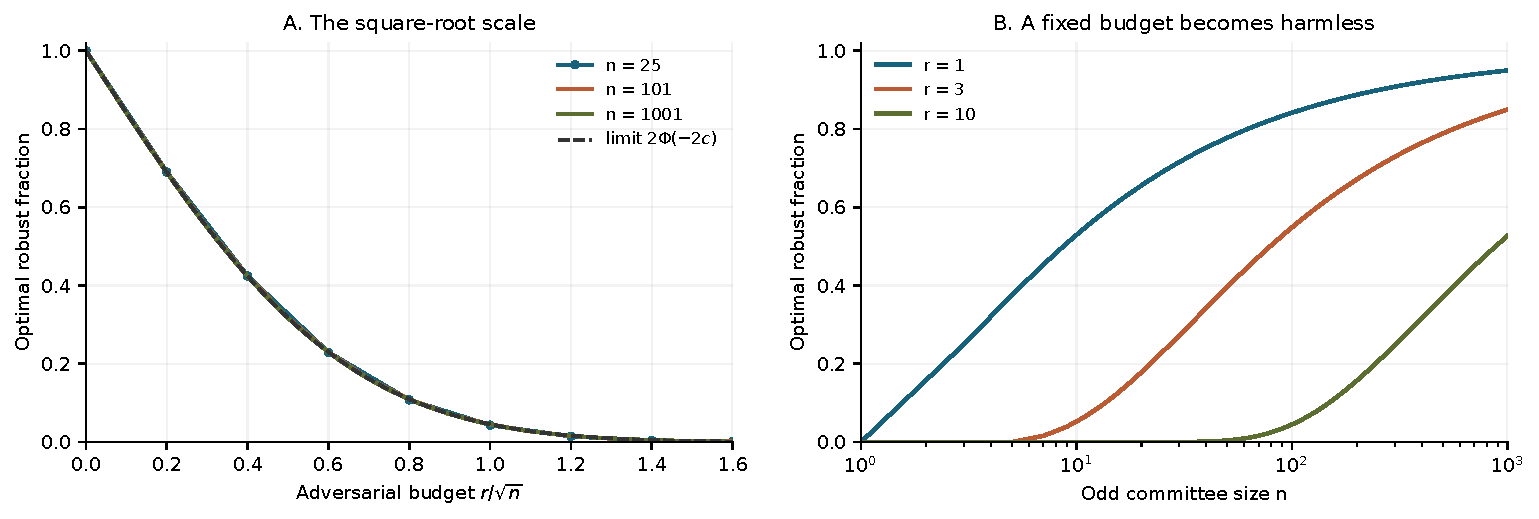
\includegraphics[width=\textwidth]{figures/robustness_profile.pdf}
\caption{Exact finite optima and their scale. Left: the binomial formula at
three odd committee sizes, plotted against \(r/\sqrt n\), with its Gaussian
limit. Right: resistance to fixed budgets improves as the committee grows.
The figure is generated from exact binomial probabilities, not Monte Carlo
estimates.}
\label{rch:fig:profiles}
\end{figure}

An elementary bound is useful for explicit extraction schedules. Put
\(c_m=\binom{2m}{m}/4^m\). Induction from
\(c_{m+1}/c_m=(2m+1)/(2m+2)\) gives
\(c_m\le1/\sqrt{m+1}\). The largest mass of
\(\operatorname{Bin}(2m+1,1/2)\) is at most \(c_m\). Therefore
\begin{equation}
 \eps_{\Maj_n}(r)\le
 \min\left\{1,\;2r\sqrt{\frac{2}{n+1}}\right\}.
 \label{rch:eq:elementarymajority}
\end{equation}
For \(r\le m\) this counts \(2r\) central masses; for larger budgets the
right-hand expression before truncation already exceeds one. In particular,
\(n+1\ge8r^2\delta^{-2}\) suffices for vulnerability at most \(\delta\).
The constant is deliberately elementary; \eqref{rch:eq:smallbudget} is sharper.

\section{A sharp inequality for what early voters can predict}
\label{rch:sec:prefix}

The key quantitative bridge does not require Kleitman's theorem. For
\(1\le m\le n\), define
\begin{equation}
 \alpha_f(m)=\left\|\E[f\mid\cF_m]\right\|_\infty.
 \label{rch:eq:alpha}
\end{equation}
This is the largest possible conditional bias after any particular assignment
of the first \(m\) votes. Also put
\begin{equation}
 \vol(m,r)=\sum_{j=0}^{\min(m,r)}\binom mj.
 \label{rch:eq:volume}
\end{equation}

\begin{theorem}[Sharp finite-prefix inequality]
\label{rch:thm:prefix}
For every neutral \(f:Q_n\to\{-1,1\}\), and every
\(1\le r\le m\le n\),
\begin{equation}
 \boxed{\quad
 \alpha_f(m)\le
 \min\left\{1,\frac{2^m}{\vol(m,r)}\eps_f(r)\right\}.
 \quad}
 \label{rch:eq:sharpalpha}
\end{equation}
The coefficient \(2^m/\vol(m,r)\) is the best possible constant independent
of the ambient dimension \(n\), for each fixed pair \((m,r)\).
In particular,
\begin{equation}
 \alpha_f(m)\le\eps_f(m),\qquad
 \alpha_f(m)\le\frac{2^m}{m+1}\eps_f(1).
 \label{rch:eq:alphaspecial}
\end{equation}
\end{theorem}

\subsection{The smallest vulnerable region in a nonconstant cube}

\begin{lemma}
\label{rch:lem:minboundary}
If \(h:Q_m\to\{-1,1\}\) is nonconstant and \(1\le r\le m\), then
\begin{equation}
 |\{x:R_h(x)\le r\}|\ge\vol(m,r).
 \label{rch:eq:minboundary}
\end{equation}
A rule with exactly one input of its minority color attains equality.
\end{lemma}

\begin{proof}
The statement for \(m=1\) is immediate, and for \(r\ge m\) every input is
vulnerable. Proceed by induction, separating the last coordinate into two
\((m-1)\)-dimensional slices.

If both slices are nonconstant, within-slice changes alone make at least
\(2\vol(m-1,r)\) vertices vulnerable. With the volume convention
\eqref{rch:eq:volume}, this is at least
\(\vol(m-1,r)+\vol(m-1,r-1)=\vol(m,r)\).

If one slice is constant, rename outputs so it is constantly positive. Let
\(A\) be the nonempty negative set in the other slice. In that other slice,
every point of its radius-\(r\) neighborhood \(N_r(A)\) is vulnerable:
positive points can reach \(A\), and negative points can move to the positive
constant slice with one change. In the constant slice, all points above
\(N_{r-1}(A)\) are vulnerable. Since a neighborhood of a nonempty set contains
a ball,
\[
 |N_r(A)|+|N_{r-1}(A)|\ge
 \vol(m-1,r)+\vol(m-1,r-1)=\vol(m,r).
\]
Oppositely colored constant slices make the entire cube vulnerable; identically
colored constant slices are excluded by nonconstancy.

Finally, if the minority set is the singleton \(\{a\}\), the vulnerable set
is exactly \(\Ball_r(a)\) for \(r\ge1\). This proves attainment.
\end{proof}

\subsection{Complementary fibres cancel}

\begin{proof}[Proof of the inequality in Theorem \ref{rch:thm:prefix}]
Write an input as \((s,y)\), where \(s\in Q_m\) is the prefix and
\(y\in Q_{n-m}\) is the tail. Let \(B\) be the set of tails for which
\(s\mapsto f(s,y)\) is nonconstant. On \(B^c\), denote its common output by
\(c(y)\).

Neutrality implies that \(B\) is invariant under \(y\mapsto-y\), and that
\(c(-y)=-c(y)\) on \(B^c\). Thus the integral of \(c\) over \(B^c\)
vanishes. For each fixed prefix \(s\),
\begin{equation}
 \left|\E_y f(s,y)\right|
 =\left|\E_y\bigl[\one_B(y)f(s,y)\bigr]\right|
 \le\Prb_y(B).
 \label{rch:eq:fibrecancel}
\end{equation}
When the tail has zero coordinates, the neutral full prefix fibre is
nonconstant, so the same argument has no homogeneous part to cancel.

By Lemma \ref{rch:lem:minboundary}, each bad tail contributes at least
\(\vol(m,r)\) prefix inputs vulnerable to \(r\) prefix changes. Such changes
are also legal changes in the whole input. Consequently
\[
 \eps_f(r)\ge\Prb_y(B)\frac{\vol(m,r)}{2^m}.
\]
Together with \eqref{rch:eq:fibrecancel}, this proves \eqref{rch:eq:sharpalpha}.
\end{proof}

\subsection{Why the constant cannot be improved}

Fix \((m,r)\) with \(1\le r\le m\). Let \(h_\ell\) be majority on an odd
number \(\ell\) of tail votes. Define
\begin{equation}
 F_\ell(s,y)=
 \begin{cases}
  1,&s=(1,\ldots,1),\\
 -1,&s=(-1,\ldots,-1),\\
 h_\ell(y),&\text{otherwise}.
 \end{cases}
 \label{rch:eq:sharpconstruction}
\end{equation}
This is neutral and \(\alpha_{F_\ell}(m)=1\). For a fixed tail, the prefix
rule is constant except for the corner forced to have the opposite output.
Its \(r\)-vulnerable prefix region has exactly \(\vol(m,r)\) points.

If \(R_{h_\ell}(y)>r\), no combination of at most \(r\) changes can alter
the tail's majority. For such a tail, the \(r\)-vulnerable prefix inputs are
exactly the radius-\(r\) ball around the exceptional corner: they can reach
that corner, or leave it if they start there. It follows that
\begin{equation}
 \frac{\vol(m,r)}{2^m}
 \le\eps_{F_\ell}(r)
 \le\frac{\vol(m,r)}{2^m}
   +\left(1-\frac{\vol(m,r)}{2^m}\right)\eps_{h_\ell}(r).
 \label{rch:eq:sharpsandwich}
\end{equation}
By Section \ref{rch:sec:scales}, the last factor tends to zero. Hence
\(\alpha_{F_\ell}(m)/\eps_{F_\ell}(r)\to2^m/\vol(m,r)\).
This proves sharpness uniformly over dimensions. It does not determine the
best constant for every fixed triple \((n,m,r)\).

\subsection{Conditional probabilities and comparisons between committees}

For every positive-probability event \(A\in\cF_m\),
\begin{equation}
 \frac{1-\alpha_f(m)}2
 \le\Prb(f=1\mid A)
 \le\frac{1+\alpha_f(m)}2.
 \label{rch:eq:history}
\end{equation}
The estimate does not deteriorate when \(A\) is a very rare prefix event.
For any earlier decision \(g:Q_m\to\{-1,1\}\),
\begin{equation}
 \left|\Prb(f=g)-\frac12\right|
 \le\frac12\alpha_f(m)
 \le\frac{2^{m-1}}{\vol(m,r)}\eps_f(r).
 \label{rch:eq:twocommittees}
\end{equation}
Indeed, \(\Prb(f=g)=(1+\E[fg])/2\), and conditional expectation bounds the
correlation. This is the precise reason strong resistance to changes in early
votes can coexist with a later decision that is almost unrelated to the earlier
one.

\section{Why increasingly resilient decisions cannot settle}
\label{rch:sec:oscillation}

Let \(f_n\) be neutral and depend on the first \(n\) inputs, and put
\(\eps_n(r)=\eps_{f_n}(r)\). Distinguish two assumptions:
\begin{align}
 \eps_n(1)&\longrightarrow0,
 &&\text{one-vote resilience;}\label{rch:eq:oneassumption}\\
 \eps_n(r)&\longrightarrow0\quad\text{for every fixed }r,
 &&\text{resilience at every fixed budget.}\label{rch:eq:allassumption}
\end{align}
The first is enough to prevent stabilization. The second allows us to arrange
almost-sure divergence of robustness along an extracted subsequence.

\begin{theorem}[Mixing and unavoidable oscillation]
\label{rch:thm:mixing}
Under \eqref{rch:eq:oneassumption}:
\begin{enumerate}[label=(\roman*)]
\item For every \(g\in L^1(\mu)\), \(\E[f_ng]\to0\).
\item For every fixed measurable \(G:\Omega\to\{-1,1\}\),
\begin{equation}
 \Prb(f_n=G)\longrightarrow\frac12.
 \label{rch:eq:nooracle}
\end{equation}
\item The decisions take both signs infinitely often on a conull, comeager set.
Their set of pointwise convergence is null and meager.
\item No deterministic infinite subsequence converges in probability.
\end{enumerate}
\end{theorem}

\begin{proof}
For each fixed \(m\), Theorem \ref{rch:thm:prefix} implies
\(\alpha_{f_n}(m)\le2^m\eps_n(1)/(m+1)\to0\). Given \(g\in L^1\),
conditional expectations on finite prefixes approximate \(g\) in \(L^1\).
More explicitly,
\begin{equation}
 |\E[f_ng]|
 \le\alpha_{f_n}(m)\|g\|_1
   +\|g-\E[g\mid\cF_m]\|_1.
 \label{rch:eq:L1estimate}
\end{equation}
First take \(n\to\infty\), then \(m\to\infty\). This proves (i), and
the identity \(\Prb(f_n=G)=(1+\E[f_nG])/2\) gives (ii).

Let \(A_+\) be the measurable event that \(f_n\) is eventually positive.
On \(A_+\), \(f_n\to1\), so dominated convergence gives
\(\E[\one_{A_+}f_n]\to\mu(A_+)\). Part (i) makes this limit zero.
Likewise the event of eventual negative output has measure zero.

For category, fix a nonempty input cylinder \(C\), determined by the first
\(m\) coordinates. For all sufficiently large \(n\),
\(\alpha_{f_n}(m)<1\), so both signs occur on \(C\). For each sign \(s\)
and each \(N\), the open set
\(\bigcup_{n\ge N}\{f_n=s\}\) is therefore dense. Intersect these sets
over \(s\) and \(N\). This gives a dense \(G_\delta\) set on which both
signs occur infinitely often.

All the arguments apply to each fixed deterministic infinite subsequence.
If such a subsequence converged in probability, a further subsequence would
converge almost surely to a measurable sign-valued limit \(G\), contradicting
\eqref{rch:eq:nooracle}. This proves (iv).
\end{proof}

Part (i) is weak-* convergence to zero in \(L^\infty\). For the sets
\(A_n=\{f_n=1\}\), it says
\begin{equation}
 \mu(A_n\cap B)\longrightarrow\tfrac12\mu(B)
 \qquad\text{for every fixed measurable }B.
 \label{rch:eq:renyi}
\end{equation}
This is mixing with density \(1/2\) in R\'enyi's terminology \cite{Renyi}.
The zero weak limit is not an admissible decision, which must be a sign.
The order of quantifiers matters: \(G\) in \eqref{rch:eq:nooracle} is fixed before
the limit. The statement is not uniform over a choice of \(G\) depending on
\(n\), and does not prohibit selecting a constant-sign subsequence after seeing
the entire input.

\subsection{An even weaker qualitative hypothesis}

Let \(x^{(i)}=\flip_i x\) denote \(x\) with coordinate \(i\) flipped, and set
\(\Inf_i(f)=\Prb(f(X)\ne f(X^{(i)}))\).

\begin{proposition}
\label{rch:prop:influences}
The conclusions of Theorem \ref{rch:thm:mixing} remain true if
\begin{equation}
 \Inf_i(f_n)\longrightarrow0\quad\text{for every fixed }i.
 \label{rch:eq:influences}
\end{equation}
\end{proposition}

\begin{proof}
For a finite nonempty set \(S\), put \(\chi_S(x)=\prod_{i\in S}x_i\).
For \(i\in S\), invariance of product measure under a coordinate flip gives
\[
 \widehat f_n(S)=\E[f_n\chi_S]
 =\tfrac12\E[(f_n-f_n\circ\flip_i)\chi_S],
\]
so \(|\widehat f_n(S)|\le\Inf_i(f_n)\to0\). Neutrality gives
\(\widehat f_n(\varnothing)=0\). The conditional expectation on a fixed
\(m\)-prefix is the finite Walsh expansion over \(S\subseteq[m]\), so its
uniform norm tends to zero. The proof of Theorem \ref{rch:thm:mixing} now applies.
\end{proof}

This statement says that if every particular early voter eventually loses
influence, no fixed measurable eventual decision can emerge. It does not say
that all small adversarial coalitions become harmless. For example,
\(f_n(x)=x_n\) satisfies \eqref{rch:eq:influences} but is always one-vote fragile.

\subsection{One-vote resilience does not imply two-vote resilience}
\label{rch:sec:separation}

There is a sharper separation between \eqref{rch:eq:oneassumption} and
\eqref{rch:eq:allassumption}. We give the construction because it rules out a
potentially misleading inference in the puzzle.

\begin{proposition}[A sharp separation of budgets]
\label{rch:prop:code}
There are neutral rules of dimensions tending to infinity for which
\(\eps_f(1)\to0\) but \(\eps_f(2)=1\) identically.
\end{proposition}

\begin{proof}
Use binary coordinates temporarily. Let \(d\ge2\), \(N=2^d-1\), and index
\(N\) coordinates by the nonzero vectors of \(\F_2^d\). Define
\[
 C=\left\{x\in\F_2^N:\sum_{v\ne0}x_vv=0\right\}.
\]
The syndrome map is surjective, so \(C\) has density \(1/(N+1)\). A
nonzero syndrome is corrected by flipping its indexed coordinate; hence every
word lies within distance one of \(C\). No nonzero codeword has weight one or
two, because the columns are nonzero and distinct. Thus the minimum distance
is at least three. Finally \(\sum_{v\ne0}v=0\), so \(C\) is invariant under
complementation.

The product \(D=C\times C\) has density \((N+1)^{-2}\), minimum distance
at least three, covering radius at most two, and is complement-invariant.
Its radius-one balls are disjoint, giving
\[
 u_N:=\Prb((X,Y)\in N_1(D))=\frac{2N+1}{(N+1)^2}.
\]
Let \(h_L\) be majority of an odd number \(L\) of further fair signs, and set
\[
 f(X,Y,Z)=h_L(Z)(-1)^{\one_D(X,Y)}.
\]
Complementation leaves \(D\) invariant and reverses \(h_L\), so \(f\) is
neutral. Every point outside \(D\) can enter it with at most two changes;
every point of \(D\) can leave with one. Thus \(R_f\le2\) everywhere.

One-change vulnerability occurs exactly when the code coordinates lie in
\(N_1(D)\), or the majority is one-change vulnerable. These events use
disjoint input coordinates. Writing \(t_L=\eps_{h_L}(1)\), we obtain
\begin{equation}
 \eps_f(1)=u_N+t_L-u_Nt_L\longrightarrow0
 \label{rch:eq:codeseparation}
\end{equation}
as \(d,L\to\infty\). Taking, for example, \(L=N\) gives the claimed
sequence of dimensions. Padding by ignored coordinates supplies a rule at
every intermediate horizon if desired.
\end{proof}

\section{Extracting a continuous open stream of almost fair decisions}
\label{rch:sec:extraction}

Oscillation alone leaves substantial freedom. We can arrange much more: a fixed
subsequence of horizons has an output law uniformly comparable with a product
of fair coins, while every output stream remains topologically attainable.

\begin{theorem}[Quantitative open recoding]
\label{rch:thm:recoding}
Suppose \(f_n\) is neutral and \(\eps_n(1)\to0\). For every \(\eta>0\)
there is a deterministic strictly increasing sequence \(n_1<n_2<\cdots\)
such that the map
\begin{equation}
 H:\Omega\longrightarrow\Omega,
 \qquad H(x)=(f_{n_j}(x))_{j\ge1}
 \label{rch:eq:H}
\end{equation}
is continuous, open, and onto. If \(\nu=H_*\mu\) and \(\beta\) is fair
product measure on the output space, then
\begin{equation}
 e^{-\eta}\beta(A)\le\nu(A)\le e^\eta\beta(A)
 \quad\text{for every Borel }A.
 \label{rch:eq:boundedmeasure}
\end{equation}
Equivalently,
\begin{equation}
 e^{-\eta}\le\frac{d\nu}{d\beta}\le e^\eta
 \quad\beta\text{-almost everywhere}.
 \label{rch:eq:density}
\end{equation}
If the stronger assumption \eqref{rch:eq:allassumption} holds, the same selection
can also ensure
\begin{equation}
 R_{f_{n_j}}(x)\longrightarrow\infty
 \quad\text{for }\mu\text{-almost every }x.
 \label{rch:eq:radiusdiverge}
\end{equation}
\end{theorem}

\subsection{The deterministic selection and the likelihood bounds}

\begin{proof}
Let \(a=1-e^{-\eta}\), and for \(j\ge2\) put
\(\delta_j=a2^{1-j}\). Thus \(0<\delta_j<1\) and
\(\sum_{j\ge2}\delta_j=a\). Choose any first horizon. Once \(n_{j-1}\)
has been chosen, take \(n_j>n_{j-1}\) so large that
\begin{equation}
 \alpha_{f_{n_j}}(n_{j-1})\le\delta_j.
 \label{rch:eq:selection}
\end{equation}
This is possible by Theorem \ref{rch:thm:prefix}. Under
\eqref{rch:eq:allassumption}, additionally require
\begin{equation}
 \eps_{n_j}(\max\{n_{j-1},j\})\le\delta_j;
 \label{rch:eq:strongselection}
\end{equation}
this stronger condition already implies \eqref{rch:eq:selection}.

The first selected output is exactly fair by neutrality. Any history of
preceding selected outputs is an event in \(\cF_{n_{j-1}}\). By
\eqref{rch:eq:history}, every next conditional probability lies between
\((1-\delta_j)/2\) and \((1+\delta_j)/2\). For every finite output word
\(b=(b_1,\ldots,b_J)\),
\begin{equation}
 \prod_{j=2}^{J}(1-\delta_j)
 \le\frac{\nu([b])}{2^{-J}}
 \le\prod_{j=2}^{J}(1+\delta_j).
 \label{rch:eq:cylinderdensity}
\end{equation}
The elementary inequalities
\[
 \prod(1-\delta_j)\ge1-\sum\delta_j=e^{-\eta},
 \qquad
 \prod(1+\delta_j)\le e^{\sum\delta_j}\le e^\eta
\]
give uniform bounds. They extend from cylinder sets and their finite unions
to all Borel sets, for example by regularity of finite measures on Cantor space.
This proves \eqref{rch:eq:boundedmeasure}, and the Radon--Nikodym theorem gives
\eqref{rch:eq:density}.

Under \eqref{rch:eq:strongselection},
\(\sum_j\Prb(R_{f_{n_j}}\le j)<\infty\). Borel--Cantelli implies that
\(R_{f_{n_j}}>j\) eventually almost surely, proving \eqref{rch:eq:radiusdiverge}.
\end{proof}

The density estimate is stronger than just convergence of finite-dimensional
distributions. It compares probabilities of \emph{all} Borel properties of the
whole output stream. In particular
\(\|\nu-\beta\|_{\TV}\le e^\eta-1\). Nevertheless, the selected outputs
need not be independent; equivalence with product measure is the claim.

\subsection{Why the decision map is open and onto}

\begin{proof}[Completion of the topological part of Theorem \ref{rch:thm:recoding}]
Every output coordinate depends on finitely many input coordinates, so \(H\)
is continuous. Let \(C\) be an input cylinder fixing the first \(k\) votes,
and choose \(J\) with \(n_J\ge k\). Fix an output word \(b\) of length
\(J\) compatible with \(C\). Then
\[
 A=C\cap\{f_{n_1}=b_1,\ldots,f_{n_J}=b_J\}
\]
is a nonempty event in \(\cF_{n_J}\), and hence has positive measure.
The conditional bounds, which are strictly between zero and one, permit either
next sign on \(A\). Repeating the argument permits every finite continuation.
The resulting nonempty closed constraints are nested in the compact input
space, so every infinite continuation is realized.

It follows that \(H(C)\) is exactly the union of the output cylinders
\([b]\) over all length-\(J\) words compatible with \(C\). This is a finite
union of cylinders, and is open. Hence \(H\) is an open map. Equation
\eqref{rch:eq:cylinderdensity} gives a preimage for every finite output word;
compactness again realizes every infinite output stream. Thus \(H\) is onto.
\end{proof}

\subsection{A coupling interpretation}

On an enlargement of the probability space, there are iid fair signs \(Z_j\)
such that, writing \(Y_j=f_{n_j}(X)\),
\begin{equation}
 \sum_{j\ge2}\Prb(Y_j\ne Z_j)
 \le\frac12\sum_{j\ge2}\delta_j<\infty.
 \label{rch:eq:coupling}
\end{equation}
One way to see this is to construct the pair sequentially. Given the already
constructed pair histories, let the next \(Y_j\) have its true conditional
Bernoulli law, which depends on the previous \(Y\)'s, and couple it maximally
with a fair \(Z_j\). The conditional mismatch probability is at most
\(\delta_j/2\), while the conditional marginal of \(Z_j\) is always fair.
This produces the prescribed law of the \(Y\)-stream and an iid \(Z\)-stream.
Standard disintegration allows the original input to be retained as well.
Borel--Cantelli then makes the two streams differ at only finitely many
positions almost surely.

The enlarged probability space is part of this coupling statement. It does not
assert that an additional independent sequence was already available as a
deterministic function of the input. The bounded-density and openness conclusions
above are direct properties of the deterministic map \(H\).

\subsection{An explicit schedule for ordinary majorities}

For \(f_n=\Maj_n\) at odd horizons, set
\(q_j=\max\{n_{j-1},j\}\). By \eqref{rch:eq:elementarymajority}, any odd
\(n_j>n_{j-1}\) satisfying
\begin{equation}
 n_j+1\ge8q_j^2\delta_j^{-2}
 \label{rch:eq:explicitschedule}
\end{equation}
meets \eqref{rch:eq:strongselection}. This produces a completely specified,
although deliberately sparse, subsequence. Finding much denser sequences with
comparably strong infinite-stream guarantees is a meaningful further problem.

\section{Opposite answers from probability and category}
\label{rch:sec:category}

Assume \eqref{rch:eq:allassumption}, and use the stronger selection in Theorem
\ref{rch:thm:recoding}. Define
\begin{equation}
 E=\{x:R_{f_{n_j}}(x)\to\infty\}.
 \label{rch:eq:E}
\end{equation}

\begin{theorem}[Two notions of typical input]
\label{rch:thm:typical}
The selected horizons have the following properties.
\begin{enumerate}[label=(\roman*)]
\item For almost every input, \(R_{f_{n_j}}\to\infty\), and the output
stream is normal: every finite sign word of length \(k\) has limiting
overlapping frequency \(2^{-k}\).
\item On a comeager set of inputs,
\begin{equation}
 \liminf_{J\to\infty}\frac1J\sum_{j=1}^J\one_{\{f_{n_j}=1\}}=0,
 \qquad
 \limsup_{J\to\infty}\frac1J\sum_{j=1}^J\one_{\{f_{n_j}=1\}}=1,
 \label{rch:eq:wildfreq}
\end{equation}
and \(R_{f_{n_j}}=1\) infinitely often.
\item The set \(E\) is Borel, conull, meager, and invariant under finite
changes and global complementation. For \(x,y\in E\),
\begin{equation}
 x\mathrel{E_0}y\quad\Longrightarrow\quad H(x)\mathrel{E_0}H(y).
 \label{rch:eq:E0hom}
\end{equation}
\end{enumerate}
\end{theorem}

\begin{proof}
The radius conclusion in (i) is \eqref{rch:eq:radiusdiverge}. Normality has full
fair-product measure. To verify this standard fact directly, fix a word of
length \(k\). Its occurrence indicators at positions in any fixed residue
class modulo \(k\) depend on disjoint input blocks and are iid with mean
\(2^{-k}\). Apply the strong law to each of the \(k\) classes, then to the
countably many words. The measure equivalence \eqref{rch:eq:density} transfers this
full-measure property to \(H(X)\).

For (ii), in the output Cantor space the set of sequences with frequencies
having liminf zero and limsup one is a dense \(G_\delta\). For example, for
each \(q,N\ge1\), the requirement that some prefix of length at least \(N\)
has positive frequency below \(1/q\) is open and dense: append a sufficiently
long block of negative signs. The analogous upper requirement is also open and
dense. Intersect them. A continuous open surjection pulls dense open sets back
to dense open sets, so \eqref{rch:eq:wildfreq} holds on a comeager input set.

For recurring fragility, fix a nonempty input cylinder \(C\). At all
sufficiently large selected horizons, both decisions occur on \(C\), since
its conditional bias is below one. The completions of \(C\) to that horizon
form a connected finite cube. A path between opposite decisions contains a
bichromatic edge, and its endpoints have \(R_f=1\). Hence, for every \(K\),
\[
 \bigcup_{j\ge K}\{x:R_{f_{n_j}}(x)=1\}
\]
is open and dense. Intersect over \(K\). This also shows that \(E\) is
meager. Its Borel character follows directly from \eqref{rch:eq:E}.

Finally, suppose \(x\) and \(y\) differ in at most \(s\) coordinates.
Whenever \(R_f(x)>s\), the outputs agree and
\begin{equation}
 R_f(y)\ge R_f(x)-s.
 \label{rch:eq:radiuslipschitz}
\end{equation}
Indeed, an opposite-output point within distance less than \(R_f(x)-s\) of
\(y\) would contradict the definition of \(R_f(x)\), by the triangle
inequality. Thus \(x\in E\) implies \(y\in E\), and the two output
streams eventually agree. Neutrality preserves all change distances under
complementation. This proves (iii).
\end{proof}

\begin{writenote}[A step made explicit, 5~October 2026]
The recurring-fragility step uses, for a cylinder $C$ fixing the first $k$
votes, that $\alpha_{f_{n_j}}(k)<1$ once $n_{j-1}\ge k$. This follows from
\eqref{rch:eq:selection} because $\alpha_f$ is nondecreasing: for
$k\le m$ the tower property gives
$\E[f\mid\cF_k]=\E\bigl[\E[f\mid\cF_m]\bigm|\cF_k\bigr]$, and conditional
expectation does not increase the uniform norm, so
$\alpha_f(k)\le\alpha_f(m)$. Hence
$\alpha_{f_{n_j}}(k)\le\alpha_{f_{n_j}}(n_{j-1})\le\delta_j<1$. Since $C$ is
an atom of $\cF_k$, the average of $f_{n_j}$ over $C$ has absolute value at
most $\alpha_{f_{n_j}}(k)<1$, so $f_{n_j}$ takes both values on $C$.
\end{writenote}

\begin{center}
\begin{tabularx}{\textwidth}{@{}P{0.25\textwidth}YY@{}}
\toprule
Property & Almost every input & A comeager set of inputs\\
\midrule
Selected decision frequencies & Every finite word has its fair frequency &
Positive frequency has liminf \(0\), limsup \(1\)\\[4pt]
Selected change distances & Tend to infinity & Equal \(1\) infinitely often\\[4pt]
Eventual decision & Does not exist & Does not exist\\
\bottomrule
\end{tabularx}
\end{center}

There is no contradiction: a conull set may be meager. Also,
\eqref{rch:eq:E0hom} is a homomorphism of equivalence relations on \(E\), not
a reduction; no converse is asserted. The restriction \(H|_E\) is not claimed
to remain open or onto.

\subsection{Why no fair-frequency conclusion holds for all horizons}

\begin{proposition}[Arbitrarily slow changes and wild full-sequence frequencies]
\label{rch:prop:slow}
There are neutral rules satisfying \eqref{rch:eq:allassumption} for which the
positive-decision frequency along \emph{all} horizons has liminf zero and
limsup one almost surely. Moreover, for any prescribed nondecreasing unbounded
function \(a:\N\to\N\), they can be chosen so that, for every input,
the number of decision changes up to horizon \(n\) is at most \(a(n)\)
for all sufficiently large \(n\).
\end{proposition}

\begin{proof}
Partition successive input coordinates into disjoint odd blocks of lengths
\(\ell_j\to\infty\), and let \(Z_j\) be their majorities. The \(Z_j\)'s
are independent fair signs. Choose deterministic release horizons \(t_j\)
so large that the first \(j\) blocks have been read by \(t_j\),
\(a(t_j)\ge j\), and \(t_{j+1}/t_j\to\infty\). Define \(f_n=Z_j\)
for \(t_j\le n<t_{j+1}\), and use \(f_n(x)=x_1\) before \(t_1\).

At each horizon the rule only uses available votes. Its robustness profile is
that of \(\Maj_{\ell_j}\), so \eqref{rch:eq:allassumption} holds. Changes can
occur only at the release horizons, with no changes before \(t_1\).
There are at most \(j\) changes during stage \(j\), which is at most
\(a(n)\) for \(n\ge t_j\). At horizon \(t_{j+1}-1\), the
last constant block of decisions occupies a fraction tending to one of the
entire elapsed time. Since the independent signs \(Z_j\) take both values
infinitely often almost surely, the full-sequence frequency approaches both
zero and one along subsequences.
\end{proof}

Thus infinite oscillation need not have a universal rate. A rate question must
also impose quantitative resilience, restrictions on ignored votes, or regular
growth conditions on the rules.

\section{A perfect infinite rule exists under choice}
\label{rch:sec:choice}

The direct infinite version asks for \(F:\Omega\to\{-1,1\}\) satisfying
\begin{equation}
 x\mathrel{E_0}y\Longrightarrow F(x)=F(y),
 \qquad F(-x)=-F(x).
 \label{rch:eq:infiniterule}
\end{equation}
The first condition says that every finite intervention is harmless, at every
input. This is an exact, global requirement, stronger than the probabilistic
finite-horizon hypotheses.

\begin{theorem}[Existence and complete failure of regularity]
\label{rch:thm:choice}
In ZFC there is an everywhere-defined rule satisfying
\eqref{rch:eq:infiniterule}. No such rule is measurable for completed fair-product
measure, and neither fibre has the Baire property. In fact both fibres have
inner measure zero and outer measure one.
\end{theorem}

\begin{proof}[Existence]
Consider the quotient set \(\Omega/E_0\). Complementation induces a
fixed-point-free involution on it: an infinite stream and its complement
disagree at every coordinate. Choose one class from each pair of complementary
classes. Give all streams in the chosen classes output \(1\), and their
complementary classes output \(-1\). This defines the required rule.
\end{proof}

This proof uses choice for a particular family of pairs; it does not identify
the assertion with full choice. Another sufficient principle is the existence
of a nonprincipal ultrafilter \(\mathcal U\) on \(\N\). Then
\begin{equation}
 F(x)=1\quad\Longleftrightarrow\quad\{i:x_i=1\}\in\mathcal U
 \label{rch:eq:ultrafilter}
\end{equation}
is neutral and finite-change invariant. It is also monotone in the votes.
This gives a concrete set-theoretic form of an infinite decision, while leaving
its exact weak-choice strength as a separate issue.

\begin{proof}[Measure obstruction]
First prove the relevant zero--one law. If a measurable set \(A\) is invariant
under finite coordinate flips, all cylinders of the same finite length have
the same conditional probability of \(A\). Thus \(A\) is independent of
every finite-prefix event, and by approximation of measurable sets by cylinder
events, it is independent of itself. Hence \(\mu(A)=\mu(A)^2\).

If \(A=F^{-1}(1)\) were measurable, this zero--one law would give
\(\mu(A)\in\{0,1\}\). Complementation preserves \(\mu\) and takes
\(A\) to \(A^c\), so neutrality instead gives \(\mu(A)=1/2\).

For the inner-measure claim, suppose a measurable \(B\subseteq A\) had
positive measure. Saturate \(B\) under the countable group of finite flips.
The saturation is measurable, invariant, still contained in \(A\), and has
measure one by the zero--one law. Its complement image is a disjoint
measure-one subset of \(A^c\), impossible. Thus \(\mu_*(A)=0\).
The same holds for \(A^c\), which implies
\(\mu^*(A)=\mu^*(A^c)=1\).
\end{proof}

\begin{proof}[Category obstruction]
An invariant set with the Baire property is either meager or comeager.
Indeed, if it is nonmeager, it is comeager inside some basic cylinder. Finite
flips take that cylinder to the finitely many cylinders of the same length
covering the whole space. Invariance makes the set comeager in each, hence
comeager globally. Neutrality interchanges the two fibres by a homeomorphism,
so they cannot be one meager and one comeager. They also cannot both be
meager or both be comeager in Cantor space. Thus neither has the Baire property.
\end{proof}

The existence of \(F\) does not contradict Theorem \ref{rch:thm:mixing}.
An arbitrary choice function can have no measurable pointwise approximation
on a positive-measure set of the specified kind. Finite combinatorial solvability
and set-theoretic existence do not by themselves provide regular limits.

\section{How a small statistical bias changes the infinite answer}
\label{rch:sec:bias}

The perfect rule remains a global object satisfying
\eqref{rch:eq:infiniterule}, but change the law of the votes. Let
\(0<p_i<1\) and
\begin{equation}
 \mu_p=\bigotimes_{i\ge1}\operatorname{Bernoulli}(p_i),
 \qquad \bar p_i=1-p_i,
 \label{rch:eq:biasedlaw}
\end{equation}
where each Bernoulli law is on \(\{-1,1\}\), assigning probability \(p_i\)
to \(1\) and probability \(1-p_i\) to \(-1\).
Neutrality still concerns renaming the alternatives; the evaluation law is
now permitted to favor one.

\begin{theorem}[Exact bias threshold]
\label{rch:thm:bias}
In ZFC, there is an everywhere-defined rule satisfying
\eqref{rch:eq:infiniterule} that is measurable for the completion of \(\mu_p\)
if and only if
\begin{equation}
 \boxed{\quad \sum_{i=1}^{\infty}(p_i-\tfrac12)^2=\infty.\quad}
 \label{rch:eq:biasthreshold}
\end{equation}
Even in the affirmative case, no such globally defined rule is Borel or has
the Baire property.
\end{theorem}

\subsection{The product-measure input}

Kakutani's theorem \cite{Kakutani} says that these two product measures are
either mutually absolutely continuous or mutually singular, and are equivalent
exactly when
\begin{equation}
 \prod_{i=1}^{\infty}2\sqrt{p_i(1-p_i)}>0.
 \label{rch:eq:kakutani}
\end{equation}
Writing \(d_i=p_i-1/2\), we have
\[
 2d_i^2\le1-\sqrt{1-4d_i^2}\le4d_i^2.
\]
For a sequence of numbers in \((0,1]\), its product is positive exactly when
the sum of its deficits from one is finite. Thus
\begin{equation}
 \mu_p\sim\mu_{\bar p}\quad\Longleftrightarrow\quad
 \sum_i d_i^2<\infty;
 \qquad
 \mu_p\perp\mu_{\bar p}\quad\Longleftrightarrow\quad
 \sum_i d_i^2=\infty.
 \label{rch:eq:productdichotomy}
\end{equation}

\begin{proof}[Proof of Theorem \ref{rch:thm:bias}]
Suppose first that the measures are equivalent. A completed-measurable
finite-change-invariant set obeys the product zero--one law, so if
\(A=F^{-1}(1)\), then \(\mu_p(A)\) is zero or one. Complementation maps
\(\mu_p\) to \(\mu_{\bar p}\) and maps \(A\) to \(A^c\). Hence
\(\mu_{\bar p}(A)=1-\mu_p(A)\), contradicting equivalence, which preserves
null and conull sets. The zero--one law here follows by deleting any finite
prefix. All sections of an exactly invariant set coincide. Since every prefix
has positive probability, completed measurability gives completed-measurable
tail sections. The set is therefore independent of every finite-prefix event;
approximation implies independence of itself. This proves the zero--one law
after completion as well.

Now suppose the measures are singular. Take a Borel set \(A_0\) with
\(\mu_p(A_0)=1\) and \(\mu_{\bar p}(A_0)=0\). Every finite flip is
nonsingular for both measures, since all coordinate probabilities are strictly
between zero and one. Intersect all finite-flip translates of \(A_0\) to
obtain a Borel, exactly finite-change-invariant set \(A\) with the same two
measure values. Let \(\kappa x=-x\) and put
\[
 A'=A\setminus\kappa A.
\]
Then \(A'\) and \(\kappa A'\) are disjoint invariant Borel sets,
\(\mu_p(A')=1\), and \(\mu_p(\kappa A')=0\). Assign opposite decisions
on these two sets. Their complement is invariant under finite changes and
under \(\kappa\), and is null for both product measures. On its remaining
complementary \(E_0\)-class pairs, use the choice construction of Theorem
\ref{rch:thm:choice}.

The resulting full-domain rule is measurable in the completion of \(\mu_p\),
because the arbitrary part lies in a Borel null set. The equivalence
\eqref{rch:eq:productdichotomy} gives \eqref{rch:eq:biasthreshold}. Global Borel or
Baire regularity is still impossible by Theorem \ref{rch:thm:choice}, independently
of which law is used to evaluate a particular completion.
\end{proof}

For example, with \(p_i=1/2+c(i+1)^{-\gamma}\), \(0<c<1/2\) and
\(\gamma\ge0\), the answer
is affirmative exactly when \(\gamma\le1/2\). An arbitrarily small bias can
therefore matter if its squared deviations accumulate without bound. This
extension is a deduction from a classical product-measure theorem, not a new
version of Kakutani's theorem. It concerns existence in one completed biased
law; it does not produce a universally measurable neutral selector.

\subsection{An explicit measurable part of the biased rule}

The conull part in the affirmative case need not be obtained by an abstract
singular-measure separator. Put \(b_i=2p_i-1\),
\[
 A_n=\sum_{i\le n}b_i^2,\qquad
 S_n(x)=\sum_{i\le n}b_ix_i,
\]
and choose \(n_j\) as the first index with \(A_{n_j}\ge j^2\). Under
\(\mu_p\), the mean of \(S_{n_j}\) is \(A_{n_j}\), and its variance is at
most \(A_{n_j}\). Hence, for every \(\epsilon>0\),
\[
 \mu_p\left(\left|\frac{S_{n_j}}{A_{n_j}}-1\right|>\epsilon\right)
 \le\frac{1}{\epsilon^2j^2}.
\]
Chebyshev's inequality and Borel--Cantelli, for rational positive \(\epsilon\),
show that \(S_{n_j}/A_{n_j}\to1\) almost surely. Under the complemented law,
the limit is \(-1\) almost surely. The two corresponding Borel limit sets are
disjoint and finite-change invariant: a finite edit changes each sufficiently
late numerator by a fixed finite amount, while the denominator diverges.
They are exchanged by complementation. Assign opposite decisions on these
two sets and use choice only on the remaining null set. This makes the
statistical part of the construction explicit.

\section{Computation, reproducibility, and the ProveIt connection}
\label{rch:sec:formal}

\subsection{What the supplied computation checks}

The accompanying \code{code/verify.py} uses integer arithmetic and the Python
standard library. It enumerates every neutral Boolean rule in dimensions one
through five. A neutral rule has one free output choice on each antipodal pair,
so the numbers of rules are
\[
 2,\quad4,\quad16,\quad256,\quad65\,536,
\]
for a total of \(65\,814\). The program computes Hamming erosions of each
positive fibre, obtaining the complete exact robustness profile. It verifies
the envelope \eqref{rch:eq:optimum} and the prefix inequalities with exact integer
comparisons. Its larger-majority tables also use exact rational values.

The successful exhaustive run includes \(394\,576\) checks of
\(\alpha_f(m)\le\eps_f(m)\), and \(985\,710\) checks of the general
volume inequality \eqref{rch:eq:sharpalpha}. These counts overlap at \(r=m\).
An independent direct minimum-Hamming-distance calculation agrees with the
erosion method for all \(278\) neutral maps in dimensions one through four.

An erosion step replaces a set \(A\) by the points whose own vertex and all
neighbors lie in \(A\). Iterating it \(r\) times gives exactly the points
whose entire Hamming radius-\(r\) ball lies in \(A\). This supplies a second
concrete view of the robust core, and an executable finite certificate.

These calculations check the finite statements and expose normalization or
off-by-one errors; they are not a replacement for the proofs in arbitrary
dimension. The probability and category theorems are proved mathematically,
not inferred from simulations. The package contains the verifier, its actual
JSON report, and the exact numerical table used for examples.

\subsection{The source snapshot and what is already formalized}

The repository inspection used the fixed ProveIt revision
\begin{center}
\small\code{3b9458b31f459b480ab43a068d7cc56f4cfdbb28}.
\end{center}
This avoids ambiguity from the actively changing main branch. The relevant
source path is
\begin{quote}\small
\path{SetTheory/Cardinals/Cardinals/Countable/GenericErgodicity.lean}.
\end{quote}
The inspected declarations include:

\begin{center}
\begin{tabularx}{\textwidth}{@{}P{0.31\textwidth}Y@{}}
\toprule
Declaration & Role in this article\\
\midrule
\code{zero_one} & Topologically transitive invariance forces a Baire set to
be meager or comeager.\\[3pt]
\code{generic_const} & A regular invariant map to a finite set is generically
constant.\\[3pt]
\code{fixed_label} & A further symmetry must fix that generic output.\\[3pt]
\code{Cantor.transitive} & Finite coordinate changes act topologically
transitively on binary streams.\\[3pt]
\code{Cantor.global_fixed_point} & An existing specialization to index
permutations and finite label actions.\\
\bottomrule
\end{tabularx}
\end{center}

The last specialization uses \emph{index permutations}; global bit
complementation is a different homeomorphism. The complement-selector
obstruction in this article follows from the abstract declarations, with that
homeomorphism supplied separately. It should not be reported as an already
named, directly matching repository theorem. The source presents proofs without
admitted statements; this investigation read the source but did not rebuild it.

The neighboring finite-symmetry file
\path{SetTheory/Cardinals/Cardinals/Combinatorics/FiniteCycles.lean}
provides additional conceptual motivation through equivariant-selector
obstructions. It is not the source of the Hamming extremum. Targeted repository
searches did not locate the quantitative robustness-to-prefix-predictability
development proved here. That is evidence about the inspected material, not
a certification of novelty across all literature or repository history.

\begin{writenote}[Checked against the repository, 5~October 2026]
At the commit this write is based on,
\path{GenericErgodicity.lean} is byte-identical to its state at the pin
(blob \file{c9b5ce93}), and so is \path{FiniteCycles.lean} (blob
\file{b1da77ef}). The five declarations of the table exist with the roles
stated, in the namespace \file{Cardinals.Countable} (the last two in its
sub-namespace \file{Cantor}); the file's header says ``Everything is proved;
nothing is admitted''; the library root
\path{SetTheory/Cardinals/Cardinals.lean} imports it; and the library's
README lists these declarations as the proved formalization of
Proposition~15.3 of the large-cardinal synthesis. No Lean build was run for
this report. \file{Cantor.global_fixed_point} does act through permutations
of the index set, and global complementation is not among the
homeomorphisms the file defines. The intake's searches found no repository
file other than this report that treats Kleitman's diameter theorem or
the worst-case (adversarial) Hamming robustness of neutral decision rules
(the only other occurrence of Kleitman's name in a report, in
\file{bounded-width-power-set-compression}, cites the Greene--Kleitman
symmetric-chain decomposition), so the statement above is still true.
\end{writenote}

\begin{remark}[{[write]} The category half from the Lean declarations, 5~October 2026]
\label{rch:rem:lean}
Identify $\Omega$ with the Cantor space $\N\to\mathrm{Bool}$ of the Lean
file, a compact Hausdorff and hence Baire space, and let $F$ satisfy
\eqref{rch:eq:infiniterule}. Suppose one fibre of $F$ has the Baire
property. The other fibre is its complement, so both fibres are Baire
measurable. (1) The finite flips \file{Cantor.flip} $S$ ($S$ a finite set
of coordinates) are homeomorphisms
acting topologically transitively (\file{Cantor.transitive}), and $F$ is
invariant under each of them by the first condition of
\eqref{rch:eq:infiniterule}; \file{generic_const} therefore gives a label
$\ell_0$ with $F=\ell_0$ on a comeager set. (2) Complementation $\kappa$ is a
homeomorphism and $F\circ\kappa=-F$ everywhere; \file{fixed_label}, applied
with $\sigma=\kappa$ and $\rho$ the negation of labels, gives
$-\ell_0=\ell_0$, which is impossible. So neither fibre has the Baire
property: this is the category half of Theorem~\ref{rch:thm:choice}, by the
route the source describes above. \emph{Formal status.} The three
declarations are proved in Lean; complementation as a Lean homeomorphism and
the assembled statement are not in the repository, so, as the source says,
this is not a named repository theorem. The measure half of
Theorem~\ref{rch:thm:choice} and every finite statement of this report have
no Lean counterpart.
\end{remark}

\subsection{A practical formalization order}

The following order separates finite algebraic obligations from measure and
category arguments.
\begin{enumerate}
\item Define neutrality, finite Hamming balls, change distance, and erosions.
Prove that robust negative cores are antipodal images of robust positive cores.
\item Formalize Lemma \ref{rch:lem:core} and the majority count. State the exact
external dependency on Kleitman's diameter theorem until that theorem itself
is formalized; do not hide it behind an unrestricted axiom.
\item Prove Lemma \ref{rch:lem:minboundary} by dimension induction. This gives a
fully elementary finite component and is well suited to independent Lean and
Rocq developments.
\item Prove the fibre-cancellation identity and Theorem \ref{rch:thm:prefix}
using finite uniform sums. Its sharpness uses only the majority estimate.
\item Transfer finite rules to product space. Establish the conditional
expectation bounds, the \(L^1\) approximation lemma, and mixing.
\item Separate the null and meager convergence proofs. Reuse the repository's
generic-ergodicity framework for the direct infinite-rule obstruction.
\item Build the deterministic extraction, cylinder likelihood estimates, and
compactness proof of openness. Formalize the finite-edit-invariant conull
domain as an additional statement, not as a claim about all inputs.
\end{enumerate}

If a family of finite truth tables is computable, the extraction indices can be
found by exhaustive search for the required rational inequalities, under the
proved promise that they eventually hold. This is an effective search procedure,
but no efficient complexity bound follows without a quantitative modulus of
resilience. For majorities, \eqref{rch:eq:explicitschedule} supplies an explicit
modulus directly.

\section{Further research questions and topics}
\label{rch:sec:questions}

The questions below extend the designed problem. A question labeled a
\emph{target} is not being asserted to be a previously published open problem;
its wider literature status requires a focused audit. The cited stability and
subsequence literature should be consulted before priority claims.

\begin{enumerate}[leftmargin=*,label=\textbf{Q\arabic*.}]
\item \textbf{Fixed-dimension sharp prefix constants.}
Determine the exact function
\[
 K(n,m,r)=\sup_{f\text{ neutral}}
 \frac{\alpha_f(m)}{\eps_f(r)}.
\]
Theorem \ref{rch:thm:prefix} determines \(\sup_{n\ge m}K(n,m,r)\), but generally
uses increasing ambient dimension for sharpness. The exact finite-dimensional
correction is a concrete extremal target amenable to certificates.

\item \textbf{Classification and stability of optimal decision rules.}
For fixed \((n,r)\), classify all neutral maximizers of \(\rho_f(r)\), then
relate near-maximal robustness to distance from a majority rule after cube
symmetries. Existing diameter stability results, including
\cite{WuEtAl}, concern the extremal cores; a full-rule classification must
also control the intervening boundary region. A statement that only repeats
known anticode stability would not constitute progress.

\item \textbf{The joint tradeoff between two intervention budgets.}
Determine attainable pairs \((\eps_f(1),\eps_f(2))\), and more generally
entire profiles, subject to neutrality and dimension. Proposition
\ref{rch:prop:code} shows that small one-vote vulnerability alone gives no
asymptotic two-vote guarantee. Quantitative restrictions on rule complexity,
monotonicity, or anonymity may restore implications.

\item \textbf{Dense extraction from majority.}
Find the slowest growth of \(n_j\) that allows the majority output law to be
equivalent to Bernoulli measure, or to have uniformly bounded density as in
\eqref{rch:eq:density}. The sufficient schedule \eqref{rch:eq:explicitschedule} is
not proposed as optimal. Distinguish equivalence of full-stream laws from
pairwise decorrelation and from a central limit theorem.

\item \textbf{A quantitative cost of changing one's mind.}
Impose a specified estimate such as
\(\eps_n(r)\le C r/\sqrt n\) over a stated range, and bound the smallest
possible number of decision changes up to horizon \(n\). Proposition
\ref{rch:prop:slow} rules out a rate theorem based only on qualitative resilience.
Restrictions requiring substantial use of all available voters may be needed.

\item \textbf{Several alternatives and other symmetry groups.}
Replace the two labels by a transitive finite group action, and formulate
neutrality so that no fixed label is allowed. The infinite generic-ergodicity
obstruction has a natural generalization, but the finite robust cores form a
multi-part packing problem. Determine which groups and alphabets admit a sharp
volume formula and a counterpart of the prefix inequality.

\item \textbf{Other adversarial metrics.}
Study weighted vote changes, interval edits, deletion/insertion distance, or
graph-local interventions. The proof strategy suggests two separate objects:
the minimum vulnerable fraction in a nonconstant fibre, and the largest
diameter or separated-core family. Identifying these two invariants may reveal
which finite--infinite conclusions survive.

\item \textbf{The exact weak-choice principle.}
Locate the existence of an everywhere neutral \(E_0\)-invariant two-label
rule among weak choice principles. Choice for the relevant quotient pairs and
a nonprincipal ultrafilter are sufficient by different constructions; no
equivalence with either is established here. Monotonicity or finite-intersection
preservation changes the question and must be specified explicitly.

\item \textbf{Beyond independent biased inputs.}
For dependent laws \(\mu\), investigate whether equivalence or singularity
of \(\mu\) and its complemented law still characterizes completed-measure
selectors. Theorem \ref{rch:thm:bias} uses both product tail triviality and
nonsingularity of finite flips. Counterexamples should isolate which of those
hypotheses fails.

\item \textbf{Effective and formal quantitative ergodicity.}
Formalize the prefix inequality, code separation, and open recoding in ProveIt.
Develop a reusable interface turning finite vulnerability bounds into measurable
and Baire nonconvergence theorems, with explicit assumptions about measure
completion and choice.
\end{enumerate}

\subsection{Further questions and research}\label{rch:sec:further}
\begin{writenote}[Added 5 October 2026, batch~114]
Following Vladimir Reshetnikov's standing rule of 4~October 2026, every
claim of the source that is not proved in full is stated here as an open
question, with its source, the argument offered and what is missing.
Questions Q1--Q10 above are the source's own research proposals, and all
ten are open. Four sentences of the body that point beyond what is proved
are attached to the question they belong to: the end of
Section~\ref{rch:sec:finite} (classification,
Question~\ref{rch:q:classify}), the end of the explicit schedule in
Section~\ref{rch:sec:extraction} (denser sequences,
Question~\ref{rch:q:dense}), the paragraph after
Proposition~\ref{rch:prop:slow} (rates, Question~\ref{rch:q:mind}) and the
``natural generalization'' of the infinite obstruction in Q6
(Question~\ref{rch:q:groups}; Proposition~\ref{rch:prop:alphabet} below
proves its regularity half). The intake found no false claim in the source.
The computations reported below were made by the write with its own
program (not shipped), an exhaustive enumeration of all $65{,}814$ neutral
rules in dimensions $1$--$5$ in exact rational arithmetic; they are
observations about those dimensions only.
\end{writenote}
\begin{enumerate}[leftmargin=*,label=\textbf{\arabic*.},ref=\arabic*]
\item\label{rch:q:constants} \textbf{Fixed-dimension prefix constants}
 (Q1). Proved: $K(n,m,r)\le2^m/\vol(m,r)$
 (Theorem~\ref{rch:thm:prefix}), and the rules $F_\ell$ show that the bound
 is the supremum over $n$. The write adds three facts with proofs.
 (a)~$K(n,m,r)$ is nondecreasing in $n$: a neutral rule on $n$ coordinates,
 read on $n+1$ coordinates by ignoring the last, is neutral, with the same
 change distances and the same $\alpha_f(m)$ for $m\le n$; so the supremum
 over $n$ is a limit. (b)~$K(n,m,r)\le1/(1-\rho_n^*(r))$, with $\rho_n^*$
 given by \eqref{rch:eq:optimum}, and equality holds for $m=n$: always
 $\alpha_f(m)\le1$, and $\eps_f(r)\ge1-\rho_n^*(r)$ by
 Theorem~\ref{rch:thm:finite}, which a maximizer attains; for $m=n$ the
 prefix determines $f$, so $\alpha_f(n)=1$ for every neutral $f$.
 (c)~$K(n,2,1)=4/3$ for $n\ge3$: majority of three votes has
 $\alpha(2)=1$ (two equal votes decide) and $\eps(1)=3/4$, so (a) gives
 $K(n,2,1)\ge4/3=2^2/\vol(2,1)$. \emph{Observation:} for every $n\le5$ and
 $1\le r\le m\le n$,
 \[
  K(n,m,r)=\min\Bigl\{\frac{2^m}{\vol(m,r)},\ \frac1{1-\rho_n^*(r)}\Bigr\},
 \]
 so the inequality of Theorem~\ref{rch:thm:prefix} is strict in those
 dimensions except when $r=m$ (both sides are $1$) or $(m,r)=(2,1)$ with
 $n\ge3$; for
 example $K(5,3,1)=8/5<2$, $K(5,4,2)=16/15<16/11$ and $K(5,5,1)=8/5<16/3$.
 Missing: whether the displayed minimum is $K(n,m,r)$ for all $n$ (the next
 dimension has $2^{32}$ neutral rules), and in any case a formula for
 $m<n$ and the rate at which $K(n,m,r)\to2^m/\vol(m,r)$.
\item\label{rch:q:classify} \textbf{Classification and stability of optimal
 rules} (Q2; the end of Section~\ref{rch:sec:finite}). Proved: majority on
 $d(n)$ coordinates attains every budget at once. Maximizers are not unique:
 composing with an isometry of the cube (a permutation of coordinates and
 sign changes of some of them) preserves neutrality and every change
 distance, and for even $n$ the ignored coordinate is arbitrary. For any
 maximizer of $\rho_f(r)$ with nonempty core, Lemma~\ref{rch:lem:core} and
 \eqref{rch:eq:corecount} make $C_r(f)$ a set of the largest size allowed by
 Theorem~\ref{rch:thm:kleitman} for diameter $n-2r-1$, so the
 characterization of those extremal families (credited to Frankl in the
 abstract of~\cite{WuEtAl}; not read by the write) describes the cores. The
 source's sketch stops there. Missing: control of the rule outside the two
 cores, which is what a classification of rules needs, and a stability
 statement for whole rules that is more than the known stability of
 cores.
\item\label{rch:q:tradeoff} \textbf{Two budgets} (Q3).
 Proved: Proposition~\ref{rch:prop:code} ($\eps(1)\to0$ with $\eps(2)=1$).
 \emph{Observation:} the attainable pairs $(\eps_f(1),\eps_f(2))$ are
 $(1,1)$ for $n=2$; $(3/4,1)$ and $(1,1)$ for $n=3$; three pairs, all with
 $\eps(2)=1$, for $n=4$; and $(5/8,15/16)$, $(3/4,1)$, $(13/16,1)$,
 $(7/8,1)$, $(15/16,1)$, $(1,1)$ for $n=5$. So in dimensions up to five a
 two-vote guarantee exists only at the smallest one-vote vulnerability,
 where majority of five attains $(5/8,15/16)$. Missing: the attainable
 region in general, and which restrictions (complexity, monotonicity,
 anonymity) force $\eps(2)\to0$ from $\eps(1)\to0$.
\item\label{rch:q:dense} \textbf{Dense extraction from majority} (Q4; the end
 of Section~\ref{rch:sec:extraction}). Proved: the schedule
 \eqref{rch:eq:explicitschedule} suffices. Since $q_j\ge n_{j-1}$ and
 $\delta_j^{-2}=4^{j-1}/a^2>1$, it forces $n_j+1\ge8n_{j-1}^2$, so
 $n_j>n_{j-1}^2$: the schedule grows at least doubly exponentially. [Sharper
 form, from the independent check of 5~October 2026: for $j\ge2$,
 $n_j\ge8n_{j-1}^2-1\ge7n_{j-1}^2$, that is, $7n_j\ge(7n_{j-1})^2$, so
 $7n_j\ge(7n_1)^{2^{j-1}}\ge7^{2^{j-1}}$.] Missing:
 any lower bound on the growth needed for bounded density
 \eqref{rch:eq:density} or for equivalence with $\beta$, and the separation
 from pairwise decorrelation and from central limit theorems.
\item\label{rch:q:mind} \textbf{A quantitative cost of changing one's mind}
 (Q5; the paragraph after Proposition~\ref{rch:prop:slow}). Proved:
 qualitative resilience gives no rate (Proposition~\ref{rch:prop:slow}).
 The source proposes assuming a bound such as $\eps_n(r)\le Cr/\sqrt n$ and
 restricting ignored votes. Missing: any rate theorem.
\item\label{rch:q:groups} \textbf{Several alternatives and other symmetry
 groups} (Q6). The source says the infinite obstruction ``has a natural
 generalization''; Proposition~\ref{rch:prop:alphabet} proves its regularity
 half for a finite alphabet and a group without a global fixed label.
 Missing: existence of such rules under choice (when an element of the group
 fixes an $E_0$-class the construction of Theorem~\ref{rch:thm:choice} does
 not apply as it stands), the finite multi-part packing problem, and an
 analogue of the prefix inequality.
\item\label{rch:q:metrics} \textbf{Other adversarial metrics} (Q7). The
 source's sketch separates two invariants: the smallest vulnerable fraction
 of a nonconstant fibre (Lemma~\ref{rch:lem:minboundary} for Hamming
 distance) and the largest separated cores (Lemma~\ref{rch:lem:core}).
 Missing: both invariants for any other metric.
\item\label{rch:q:weakchoice} \textbf{The exact weak-choice principle} (Q8).
 Proved: choice for the pairs of complementary $E_0$-classes, or a
 nonprincipal ultrafilter on $\N$, suffices. The write notes that the first
 is also necessary, over ZF: a rule $F$ satisfying
 \eqref{rch:eq:infiniterule} is constant on each $E_0$-class and takes
 opposite values on complementary classes, so the classes on which $F=1$
 select one class from each complementary pair. The question is therefore
 where this selection principle lies among weak choice principles (the
 sibling \file{noisy-parity-cubes}, \file{np:found:choice}, records the
 analogous equivalence for parity labels and a model of Serafin separating
 it from ultrafilters and $E_0$-transversals). Missing: that placement.
\item\label{rch:q:dependent} \textbf{Beyond independent biased inputs} (Q9).
 Theorem~\ref{rch:thm:bias} uses the zero--one law for finite-change
 invariant sets and nonsingularity of finite flips. Missing: a criterion for
 dependent laws, or counterexamples isolating the hypothesis that fails.
\item\label{rch:q:formal} \textbf{Effective and formal quantitative
 ergodicity} (Q10). Remark~\ref{rch:rem:lean} shows what the existing Lean
 declarations give. The formalization order of Section~\ref{rch:sec:formal}
 is a proposal. Missing: every formal statement of this report.
\end{enumerate}

\begin{proposition}[{[write]} Several labels: the regularity obstruction, 5~October 2026]
\label{rch:prop:alphabet}
Let $\Sigma$ be a finite set with at least two elements, and let a group
$G$ act on $\Sigma$ so that no element of $\Sigma$ is fixed by all of $G$.
Let $G$ act on $\Sigma^{\N}$ coordinatewise, and give $\Sigma^{\N}$ the
product topology and the uniform product measure $\lambda$. Suppose
$F:\Sigma^{\N}\to\Sigma$ satisfies $F(x)=F(y)$ whenever $x$ and $y$ differ
in finitely many coordinates, and $F(gx)=gF(x)$ for all $g\in G$ and all
$x$. Then the fibres of $F$ are not all measurable for the completion of
$\lambda$, and they do not all have the Baire property. If $G$ acts
transitively on $\Sigma$, no fibre is measurable and no fibre has the Baire
property.
\end{proposition}

For $\Sigma=\{-1,1\}$ and $G=\{\pm1\}$ acting by multiplication this gives
the nonmeasurability and the Baire-property statement of
Theorem~\ref{rch:thm:choice}, without its inner- and outer-measure
refinement.

\begin{proof}
Write $A_s=F^{-1}(s)$. For $k\ge1$ and a permutation $\pi$ of $\Sigma^k$, let
$\phi_\pi$ replace the first $k$ coordinates $w$ of a point by $\pi(w)$.
Each $\phi_\pi$ is a homeomorphism preserving $\lambda$ and changes only
finitely many coordinates, so every fibre is invariant under all
$\phi_\pi$; for each $k$ these maps act transitively on the cylinders
$[w]$, $w\in\Sigma^k$.

\emph{Zero--one laws.} Let $A$ be invariant under all $\phi_\pi$. If $A$ is
measurable for the completion, then $\lambda(A\cap[w])$ is the same for all
$w\in\Sigma^k$, so $\lambda(A\cap[w])=\lambda(A)\lambda([w])$. The
cylinders and $\varnothing$ form a $\pi$-system generating the Borel sets,
so $A$ is independent of every Borel set; choosing a Borel $B$ with
$\lambda(A\triangle B)=0$ gives $\lambda(A)=\lambda(A\cap B)=\lambda(A)^2$,
so $\lambda(A)\in\{0,1\}$. If $A$ has the Baire property and is not meager,
it is comeager in some cylinder $[w]$; each $[w']$ with $w'$ of the same
length is the image of $[w]$ under some $\phi_\pi$, which maps $A$ to
itself, so $A$ is comeager in each of these finitely many cylinders, which
cover $\Sigma^{\N}$, and $A$ is comeager.

\emph{The fibres.} For $g\in G$ the map $x\mapsto gx$ is a homeomorphism
preserving $\lambda$ (it permutes the letters of each coordinate), and it
maps $A_s$ onto $A_{gs}$, since $F(gx)=gF(x)$. If all fibres are
measurable, they are disjoint, cover the space and have measure $0$ or $1$,
so exactly one, $A_{s_0}$, has measure one; then $A_{gs_0}=gA_{s_0}$ has
measure one, so $gs_0=s_0$ for every $g$, contrary to the hypothesis. If all
fibres have the Baire property, each is meager or comeager; they are not all
meager, since finitely many meager sets cannot cover the compact Hausdorff,
hence Baire, space $\Sigma^{\N}$, and two disjoint sets cannot both be
comeager; so exactly one, $A_{s_0}$, is comeager, and
$A_{gs_0}=gA_{s_0}$ is comeager, so again $gs_0=s_0$ for every $g$. If $G$
acts transitively and one fibre $A_s$ is measurable (or has the Baire
property), then so is every $A_{gs}=gA_s$, that is, every fibre, and the
previous case applies.
\end{proof}

\begin{writenote}[Independent check of the write, 5 October 2026]
An adversarial check made by the intake after the write (commit
\file{9ccf04eae}) found no item needing a correction. It reread the proof of
Proposition~\ref{rch:prop:alphabet} line by line: the prefix maps
$\phi_\pi$ preserve $\lambda$ and every fibre; both zero--one laws are
proved inside the proof (a Dynkin-system argument for the measure, finitely
many cylinders for category), so no external ergodicity or Hewitt--Savage
theorem is used; $G$ may be infinite; and the specialization to
Theorem~\ref{rch:thm:choice} is correct. (The check suggested remarking that
$\lvert\Sigma\rvert\ge2$ follows from the hypothesis on $G$. That holds only
for nonempty $\Sigma$: for $\Sigma=\varnothing$ the hypothesis on $G$ holds
vacuously, $F$ is the empty map and there are no fibres. The statement is
left as it is.) It confirmed Remark~\ref{rch:rem:lean} against
\file{SetTheory/Cardinals/Cardinals/Countable/GenericErgodicity.lean} at
commit \file{74a988c32} (the three declarations and their hypotheses, and
that no other Lean file uses them, so the assembled statement is not a
repository theorem); re-derived facts (a)--(c) of
item~\ref{rch:q:constants}; and, with its own program (exact rational
arithmetic over all $65{,}814$ neutral rules of dimensions $1$--$5$, written
independently of the write's; not shipped), reproduced the displayed
formula for $K(n,m,r)$ in all $35$ cases $1\le r\le m\le n\le5$, the three
printed values, the equality cases of Theorem~\ref{rch:thm:prefix} and every
list of attainable pairs in item~\ref{rch:q:tradeoff}. It confirmed the
growth bound of item~\ref{rch:q:dense} (the sharper form recorded there is
the check's), the ZF equivalence of item~\ref{rch:q:weakchoice}, and the
note on Huang, Klurman and Pohoata against arXiv:1812.05989v1 (Theorem~1.1
with its two bounds, their sharpness and the extremal sets, the attribution
to Kleitman, and the entry ``J. Combin. Theory Ser. A 43 (1986)'' in that
paper's bibliography), together with the identity behind
\eqref{rch:eq:kleitodd}.
\end{writenote}

\clearpage
\appendix
\section{A concise problem statement suitable for sharing}

\begin{quote}
For every positive integer \(n\), a committee rule receives \(n\) signs and
returns one sign. Reversing every input sign must reverse its answer. Under
uniform random input, call a configuration \(r\)-safe if no adversary changing
at most \(r\) signs can change the answer.

Find the largest possible fraction of \(r\)-safe configurations, including the
even/odd dependence. Then evaluate a neutral rule at each successive prefix of
one infinite fair stream. Suppose, for every fixed \(r\), the probability of
being \(r\)-safe tends to one. Can the answers eventually settle with positive
probability? Can they settle on a nonmeager set? Can a perfectly safe neutral
answer be assigned directly to every infinite stream? Finally, determine whether
one can select fixed committee sizes along which decisions behave statistically
like an infinite fair-coin sequence while individual finite interventions
eventually become harmless almost surely.
\end{quote}

The finite answer is \eqref{rch:eq:optimum}. Stabilization is impossible in both
regularity senses. A direct everywhere assignment exists under choice and lacks
both regularities. The selected-size statistical assertion holds in the precise
bounded-density and coupling senses of Section \ref{rch:sec:extraction}.

\section{Scope and assumptions at a glance}

\begin{center}
\begin{tabularx}{\textwidth}{@{}P{0.29\textwidth}YY@{}}
\toprule
Statement & Essential assumptions & Nature of the result\\
\midrule
Finite optimum & Uniform finite cube; pointwise neutrality & Corollary of
Kleitman, with full reduction and matching construction\\[4pt]
Sharp prefix inequality & Uniform finite cube; pointwise neutrality &
Elementary proof and asymptotically matching examples\\[4pt]
No measurable limit & Vanishing one-vote vulnerability, or vanishing influence
of each fixed coordinate & Direct proof of a R\'enyi mixing consequence\\[4pt]
Open near-Bernoulli recoding & Vanishing finite-prefix conditional biases &
Deterministic subsequence, full-stream density comparison\\[4pt]
Diverging selected robustness & Vulnerability tends to zero for every fixed
budget & Borel--Cantelli and finite-change invariance on a conull set\\[4pt]
Perfect infinite selector & A sufficient choice principle & Exists globally;
fair-product and Baire regularity impossible\\[4pt]
Biased-law threshold & Independent nondegenerate coordinates; ZFC; completed
measurability & Corollary of Kakutani with a global choice extension\\
\bottomrule
\end{tabularx}
\end{center}

If external randomness is introduced, neutrality should hold for each fixed
seed. A distributionally neutral rule could simply use a single external fair
coin forever and ignore the votes, which changes the problem. A mixture of
fixed-seed neutral finite rules cannot exceed the deterministic finite optimum
for the averaged robustness objective, because each seed already obeys that
bound.

\begin{thebibliography}{99}
\raggedright

\bibitem{Epoch}
T. Besiroglu, E. Glazer, and C. Falkman Olsson,
\emph{FrontierMath: A benchmark for evaluating advanced mathematical reasoning
in AI}, Epoch AI, 8 November 2024, author biography for Elliot Glazer.
\url{https://epoch.ai/frontiermath/tiers-1-4/the-benchmark}.
Accessed 5 October 2026.

\bibitem{Glazer}
E. Glazer,
\emph{Interactions Among Principles of Choice, Forcing, and Measure Theory},
Ph.D. dissertation, Harvard University, September 2023.
\url{https://dash.harvard.edu/server/api/core/bitstreams/a9e00aca-1b33-41ea-bba3-2b464566635d/content}.
See especially the abstract and Section 4.4.

\bibitem{ProveIt}
V. Reshetnikov et al., \emph{ProveIt}, source repository, revision
\code{3b9458b31f459b480ab43a068d7cc56f4cfdbb28}, inspected 5 October 2026.
\url{https://github.com/VladimirReshetnikov/ProveIt}.
Relevant file: \path{SetTheory/Cardinals/Cardinals/Countable/GenericErgodicity.lean}.

\bibitem{Kleitman}
D. J. Kleitman, On a combinatorial conjecture of Erd\H{o}s,
\emph{Journal of Combinatorial Theory} \textbf{1}(2) (1966), 209--214.
\href{https://doi.org/10.1016/S0021-9800(66)80027-3}{doi:10.1016/S0021-9800(66)80027-3}.

\bibitem{HKP}
H. Huang, O. Klurman, and C. Pohoata,
\emph{On subsets of the hypercube with prescribed Hamming distances},
arXiv:1812.05989, 2018. Theorem 1.1 gives both parities of the diameter bound.
\url{https://arxiv.org/abs/1812.05989}.
Author-hosted manuscript:
\url{https://www.math.emory.edu/~hhuan30/papers/kleitman_HKP.pdf}.

\bibitem{Renyi}
A. R\'enyi, On mixing sequences of sets,
\emph{Acta Mathematica Academiae Scientiarum Hungaricae} \textbf{9} (1958),
215--228. \href{https://doi.org/10.1007/BF02023873}{doi:10.1007/BF02023873}.
\url{https://static.renyi.hu/renyi_cikkek/1958_on_mixing_sequences_of_sets.pdf}.

\bibitem{Aldous}
D. J. Aldous, Limit theorems for subsequences of arbitrarily-dependent
sequences of random variables,
\emph{Zeitschrift f\"ur Wahrscheinlichkeitstheorie und verwandte Gebiete}
\textbf{40}(1) (1977), 59--82.
For broader context see also his \emph{Exchangeability and Related Topics},
1985, \url{https://www.stat.berkeley.edu/~aldous/Papers/me22.pdf}.

\bibitem{AldousEagleson}
D. J. Aldous and G. K. Eagleson, On mixing and stability of limit theorems,
\emph{Annals of Probability} \textbf{6}(2) (1978), 325--331.
\href{https://doi.org/10.1214/aop/1176995577}{doi:10.1214/aop/1176995577}.

\bibitem{Kakutani}
S. Kakutani, On equivalence of infinite product measures,
\emph{Annals of Mathematics} (2) \textbf{49}(1) (1948), 214--224.
\href{https://doi.org/10.2307/1969123}{doi:10.2307/1969123}.
\url{https://www.jstor.org/stable/1969123}.

\bibitem{WuEtAl}
Y. Wu, Y. Li, L. Feng, J. Liu, and G. Yu,
\emph{Stabilities of the Kleitman diameter theorem},
arXiv:2411.08325v2, revised 10 June 2025.
\url{https://arxiv.org/abs/2411.08325v2}.

\end{thebibliography}
\end{document}
